\cotefile{138}
\scanpage{1}
\begin{center}
{\Huge\sffamily IMAG}\\[1ex]
{\sffamily INSTITUT MONTPELLIERAIN}\\
{\sffamily ALEXANDER GROTHENDIECK}
\end{center}
\figure{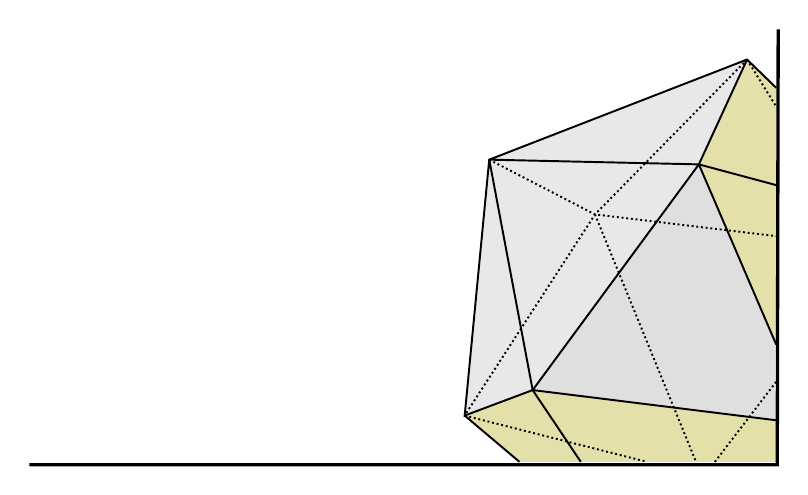
\begin{tikzpicture}[x=.012cm,y=-.012cm,line width=.7pt]
\fill[gray!18] (497,138)--(770,32)--(719,143)--(543,382)--(471,409)--cycle;
\fill[gray!25] (719,143)--(800,334)--(800,414)--(543,382)--cycle;
\fill[olive!25] (770,32)--(801,62)--(801,165)--(719,143)--cycle;
\fill[olive!25] (719,143)--(801,165)--(801,334)--cycle;
\fill[olive!25] (471,409)--(543,382)--(801,414)--(801,458)--(529,458)--cycle;
\draw (497,138)--(770,32)--(801,62) (770,32)--(719,143)--(497,138)--(471,409)--(543,382)--(497,138);
\draw (719,143)--(543,382)--(801,414) (719,143)--(801,165) (719,143)--(801,334) (471,409)--(529,458) (543,382)--(594,458);
\draw[densely dotted] (497,138)--(609,196)--(801,219) (770,32)--(609,196)--(471,409) (609,196)--(716,458) (471,409)--(664,458) (736,458)--(801,373) (770,32)--(801,82);
\draw[line width=1.2pt] (10,461)--(802,461)--(803,0);
\end{tikzpicture}}

\scanpage{2}
% archive foliation: 1
\begin{center}\textbf{\Large COMMUNIQUE DE TOPOLOGIE STRUCTURALE}\end{center}

Le numéro 4 du bulletin est actuellement sous presse. Voici quelques exemples de ce que vous y trouverez.

\begin{minipage}[t]{.50\linewidth}
\textbf{Alan Holden} (New Jersey, USA) nous montre comment lier les anneaux polygonaux des tiges pour obtenir des formes polyédriques rigides. Exposant diverses possibilités à l'aide d'illustrations saisissantes de ses maquettes, il défie les lecteurs d'en trouver d'autres.

\textbf{David Georges Emmerich et Didier Aubry}, architectes à l'Ecole nationale supérieure des Beaux-Arts, Paris, étudient les empilements concentriques des polyèdres réguliers. De tels arrangements laissent des vides qui peuvent eux-mêmes être considérés comme étant des «polyèdres mixtes» dont les faces sont soit planes soit arrondies, bordées par des polygones réguliers (plans ou gauches).

\textbf{Michael Goldberg} (Washington DC, USA), mathématicien spécialisé dans l'étude des chaînons mécaniques, des rotors, des polyèdres et de leurs possibilités de juxtaposition, remanie son «autobiographie mathématique». A propos, un rotor est un ovale non circulaire capable de se mouvoir à l'intérieur d'un polygone régulier, entrant en contact avec tous ses côtés.

Reconsidérant ses études fort renommées sur les \unsure{zonaèdres|zonoèdres}, \textbf{Anton Hanegraaf} (Elst, Pays-Bas) nous invite à examiner un ensemble fascinant de vingt problèmes combinatoires.

Dans certaines positions, une structure normalement rigide, même isostatique, subit des mouvements finis ou infinitésimaux. \textbf{Ben Roth} (University of Wyoming, USA) formule une série de questions mathématiques concernant ces situations «particulières», et des fonctions d'énergie associées.

Du Form Studies Unit à Carleton University, Canada, \textbf{Gulzar Haider} nous parle des chaînons polyédriques et de leurs réseaux connexes, ainsi que de leurs applications architecturales.

\textbf{Tibor Tarnai}, du Hungarian Institute for Building Science, analyse, de son point de vue d'ingénieur, la rigidité des cylindres en treillis et réseaux munis de sommets sur la sphère.

On peut construire des polyèdres (et ensembles de polyèdres) ayant le même type de face, en fixant face à face des dodécaèdres réguliers. \textbf{Koji Miyazaki et Ichiro Takada} (Kobe University, Japon) nous présentent leur merveilleux travail magnifiquement illustré.
\end{minipage}\hfill
\begin{minipage}[t]{.46\linewidth}
\figure{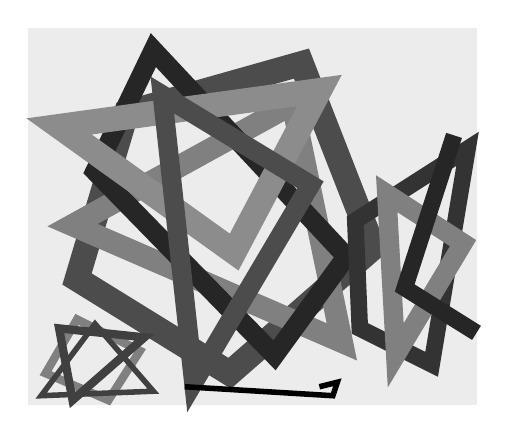
\begin{tikzpicture}[x=.57cm,y=.57cm]
\fill[gray!15] (0,0) rectangle (10,8.4);
\begin{scope}[line cap=butt,line join=miter]
\draw[black!70,line width=9pt] (1.1,2.8)--(2.2,6.5)--(6.1,7.6)--(7.7,3.5)--(4.5,.7)--cycle;
\draw[black!50,line width=8pt] (1.0,4.0)--(5.9,6.7)--(7.0,1.4)--cycle;
\draw[black!85,line width=7pt] (2.8,7.9)--(1.5,5.2)--(5.5,1.1)--(7.1,3.3)--cycle;
\draw[black!45,line width=9pt] (.7,6.2)--(4.6,3.4)--(6.5,7.0)--cycle;
\draw[black!70,line width=7pt] (3.0,6.9)--(6.3,4.9)--(3.7,.5)--cycle;
\draw[black!80,line width=6pt] (7.3,4.1)--(9.8,5.7)--(9.0,.9)--(7.4,1.7)--cycle;
\draw[black!50,line width=7pt] (8.0,4.7)--(9.7,3.6)--(8.2,1.1)--cycle;
\draw[black!85,line width=6pt] (9.5,6.0)--(8.4,2.6)--(10,1.6);
\draw[gray,line width=3pt] (.4,.7)--(1.1,1.9)--(2.5,1.2)--(1.8,.1)--cycle;
\draw[black!75,line width=2pt] (.3,.2)--(1.5,1.8)--(2.8,.3)--cycle;
\draw[black!75,line width=3pt] (.7,1.7)--(1.0,.1)--(2.6,1.5)--cycle;
\draw[line width=2pt] (3.5,.4)--(6.8,.2)--(6.9,.5)--(6.5,.4);
\end{scope}
\end{tikzpicture}}
% crop-candidate: scan 2

\figure{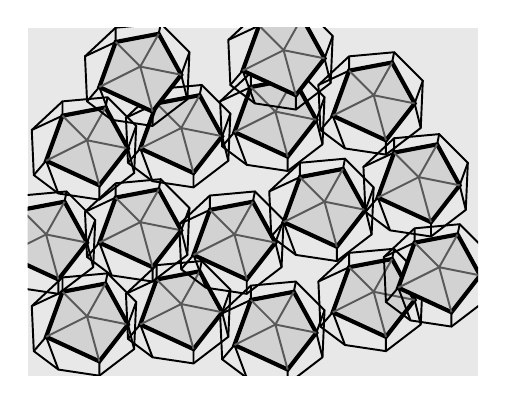
\begin{tikzpicture}[x=.52cm,y=.52cm,line width=.7pt]
\clip (0,0) rectangle (11,8.5);
\fill[gray!18] (0,0) rectangle (11,8.5);
\foreach \x/\y in {1.4/1.2,3.7/1.5,6/1,8.4/1.8,10/2.4,.4/3.2,2.7/3.5,5/3.2,7.2/4,9.5/4.6,1.4/5.5,3.7/5.8,6/6.2,8.4/6.6,2.7/7.3,6.2/7.7}{
\begin{scope}[shift={(\x,\y)}]
\fill[gray!35] (-.95,-.25)--(-.55,.85)--(.5,1.05)--(1.05,.05)--(.35,-.85)--cycle;
\draw (-1.25,-.6)--(-1.3,.5)--(-.55,1.2)--(.55,1.3)--(1.25,.6)--(1.2,-.55)--(.35,-1.2)--(-.65,-1.05)--cycle;
\draw[line width=1.5pt] (-.95,-.25)--(-.55,.85)--(.5,1.05)--(1.05,.05)--(.35,-.85)--cycle;
\draw (-1.25,-.6)--(-.95,-.25) (-1.3,.5)--(-.55,.85) (-.55,1.2)--(-.55,.85) (.55,1.3)--(.5,1.05) (1.25,.6)--(1.05,.05) (1.2,-.55)--(1.05,.05) (.35,-1.2)--(.35,-.85) (-.65,-1.05)--(-.95,-.25);
\draw[black!65] (-.55,.85)--(.05,.25)--(.5,1.05) (.05,.25)--(1.05,.05) (.05,.25)--(.35,-.85) (.05,.25)--(-.95,-.25);
\end{scope}}
\end{tikzpicture}}
% crop-candidate: scan 2
\end{minipage}

Topologie Structurale est un nouveau champ de recherche interdisciplinaire, faisant appel au talent de mathématiciens, architectes et ingénieurs, collaborant à sa réussite. Nous vous invitons à vous joindre aux efforts du groupe, et à communiquer vos idées en les publiant dans le bulletin. Si vous n'y êtes pas déjà abonné, pourquoi attendre? Faites-le dès aujourd'hui. Et si votre bibliothèque ne connaît pas encore Topologie Structurale, parlez-en au bibliothécaire sans plus tarder. Nous vous en serions très reconnaissants.

\scanpage{3}
% archive foliation: 2
\textbf{Poly-kit}, premier d'une série de jeux éducatifs a obtenu un grand succès dans bon nombre de milieux, auprès de personnes de tout âge, et dans maints pays. \textbf{Lionel March} (Centre for Configurational Studies, Open University, G-B) écrit:

\textit{Le Poly-kit de Janos Baracs remporte un énorme succès dans une école primaire de chez nous. Tous les enseignants en parlent et sa réputation ne cesse de grandir. Je pense moi-même que le Poly-kit pourrait être utilisé lors de nos propres cours donnés à l'Open University.}»

Poly-kit permet de construire tous les polyèdres réguliers et semi-réguliers et certains de leurs duals. (Pour de plus amples informations, voir p. 75 de T.S. n° 1 ou p. 66 de T.S. n° \unsure{3..)|3.)}

Les numéros précédents 1, 2 et 3 publiés en 1979 sont toujours disponibles. Certains articles des numéros 2 et 3 étaient axés sur certains cas spécifiques des domaines de l'architecture et du génie et principalement sur une approche modulaire du design urbain et les systèmes d'immeubles industrialisés. D'autres articles faisaient ressortir les questions mathématiques prédominantes qui se distinguent dans cette recherche.

Déjà, en cette seconde année de publication de la revue, l'échange des résultats de recherche et des problèmes pendants du domaine de la topologie structurale ont atteint un niveau très satisfaisant. Nous sommes très heureux de pouvoir compter sur la collaboration de tant de mathématiciens, architectes et ingénieurs intéressés par le sujet si intrigant et si passionnant qu'est la topologie structurale et de pouvoir ainsi nous adresser à vous directement par le biais du bulletin. Certains d'entre vous peuvent désirer consulter tout simplement Topologie Structurale à la Bibliothèque au lieu de s'abonner personnellement. Dans ce cas, veuillez indiquer sur la carte-réponse ci-dessous que vous aimeriez figurer sur notre liste d'envoi, uniquement pour les nouvelles. Nous désirons maintenir le contact avec vous.

\noindent\dotfill

\noindent N° d'abonné (si nécessaire) \underline{\hspace{1cm}}\hfill\textbf{\Large Topologie Structurale}

Nom et adresse du demandeur:
\begin{center}
\rule{.8\linewidth}{.4pt}\\[1ex]
\rule{.8\linewidth}{.4pt}\\[1ex]
\rule{.8\linewidth}{.4pt}\\[1ex]
\rule{.8\linewidth}{.4pt}\\[1ex]
\rule{.8\linewidth}{.4pt}
\end{center}

Veuillez m'envoyer:
\diagram{\[\begin{array}{llcc}
&&\text{Individuel}&\text{Institution}\\
\square&\text{Abonnement à Topologie structurale pour 1980 (N°s 4-6)}\ \cdots&\$20&\$30\\
\square&\text{Numéros précédents publiés en 1979 (1-3)*}\ \cdots&\$20&\$30\\
\square&\text{Numéro individuel:}\quad\square\ \#1^*\quad\square\ \#2\quad\square\ \#3\ \cdots\ \text{chacun}&\$10&\$15\\
\square&\text{Poly-kits. Combien?}\ \underline{\hspace{1cm}}\ \cdots\ \text{chacun}&\$10&\$10\\
&\hfill\text{*si disponible}&&
\end{array}\]}

$\square$ Veuillez m'inscrire sur votre liste d'envoi pour les nouvelles.\\
$\square$ Montant total joint:\underline{\hspace{1cm}} s.v.p. établir vos chèques au nom de «Topologie Structurale».\\
$\square$ Veuillez me facturer.

\noindent\textbf{\Large Adresser à}\hfill
\begin{tabular}{c}
Topologie Structurale, Ecole d'Architecture, Université de Montréal\\
Montréal, Québec, H3C 3J7, Canada
\end{tabular}

\figure{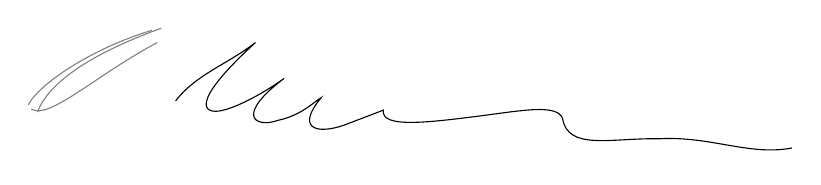
\begin{tikzpicture}[x=.013cm,y=.013cm]
\draw[gray] (0,30) .. controls (10,50) and (61,85) .. (121,103);
\draw[gray] (9,23) .. controls (21,55) and (69,83) .. (130,105);
\draw[gray] (3,26) .. controls (20,15) and (66,59) .. (126,91);
\draw (144,34) .. controls (164,60) and (195,70) .. (222,91) .. controls (166,40) and (166,22) .. (186,24) .. controls (205,27) and (235,45) .. (250,56) .. controls (202,20) and (221,7) .. (244,15) .. controls (267,20) and (279,33) .. (286,37) .. controls (259,4) and (286,1) .. (313,12) -- (347,25) .. controls (344,7) and (391,13) .. (439,19) .. controls (485,25) and (516,31) .. (522,17) .. controls (527,-15) and (570,-2) .. (616,-3) .. controls (666,0) and (705,-20) .. (746,-12);
\end{tikzpicture}}

\scanpage{4}
% archive foliation: 3
\begin{flushright}
\unsure{dictionnaire} \unsure{galoisien}\\
de \unsure{descente} \unsure{etc\ldots}
\end{flushright}

\scanpage{5}
% archive foliation: 4
\textcircled{1.1.}
\[
(1)\quad\left\{\begin{array}{l}
k\ \text{corps}\\
\bar k\ \text{clôture séparable},\quad \Gamma=\deleted{\unsure{\operatorname{Aut}_k}}\operatorname{Gal}(\bar k/k)\quad\text{(groupe profini)}
\end{array}\right.
\]
\[
(2)\quad\left\{\begin{array}{l}
\mathcal X\ \text{schéma connexe sur }\bar k\\
\mathcal G=\operatorname{Aut}_k(\mathcal X)\\
\mathbb G=\operatorname{Aut}_{\bar k}(\mathcal X)
\end{array}\right.
\]
\margin{On suppose que $\bar k$ est séparablement clos dans $H^0(\mathcal X,\mathcal O_{\mathcal X})$ donc $\bar k$ est la clôture séparable de $k$ dans $H^0(\mathcal X,\mathcal O_{\mathcal X})$}
\[
(3)\quad\boxed{\diagram{\begin{tikzcd}[ampersand replacement=\&]
1\ar[r]\&\mathbb G\ar[r]\&\mathcal G\ar[r]\&\Gamma.
\end{tikzcd}}}
\]

\textcircled{1.2} Si $k\subset\unsure{k'_1|k_1}\subset\bar k$, alors $\unsure{k'_1|k_1}\longleftrightarrow\Gamma_1$ sous-groupe fermé de $\Gamma$
\[
(4)\quad \boxed{\unsure{\mathcal G'_1|\mathcal G_1}=\operatorname{Aut}_{k_1}(\mathcal X)}
\]
est donc l'image inverse de $\deleted{\unsure{\mathcal G}}\Gamma$ dans $\mathcal G$.
\[
(5)\quad\diagram{\begin{tikzcd}[ampersand replacement=\&]
1\ar[r,no head]\&\mathbb G\ar[r,no head]\&\mathcal G\ar[r]\&\Gamma\\
1\ar[r,no head]\&\mathbb G\ar[u,equal]\ar[r,no head]\&\mathcal G_1\ar[u,hook,"\unsure{\mathrm{cont}}"']\ar[r]\&\Gamma_1\ar[u,hook]
\end{tikzcd}}
\]

\textcircled{1.3} Une donnée de descente \deleted{\unsure{sur}} $\mathcal X$ de $\bar k:k$ revient à un scindage de 3,
\[
(6)\quad\diagram{\begin{tikzcd}[ampersand replacement=\&]
1\ar[r]\&\mathbb G\ar[r,no head]\&\mathcal G\ar[r,no head]\&\Gamma\ar[r,"!"]\ar[l,bend left=50]\&1
\end{tikzcd}}
\]
qui permet d'écrire
\[
(7)\qquad \mathcal G\simeq\Gamma\mathbin{\underset{\scriptscriptstyle1/2}{.}}\mathbb G
\]
Donc sous réserve (\inserted{de conditions} d'effectivité, \deleted{\unsure{et ceci}} \unsure{Ch 2.} $\mathcal X$ quasi-projectif sur $\bar k$) il revient au $=$ de se donner un couple $X/k$ et un iso
\[
(8)\qquad X\otimes_k\bar k\simeq\mathcal X
\]

\scanpage{6}
% archive foliation: 5
\textcircled{1.3.1.} Plus \unsure{gén.}, une descente de $\mathcal X$ au corps de base $k'$ revient à un \inserted{$\Gamma'$-}scindage
\[
(9)\quad\diagram{\begin{tikzcd}[ampersand replacement=\&]
\mathcal G\ar[r]\&\Gamma\\
\&\Gamma_1\ar[u,hook]\ar[ul,dashed]
\end{tikzcd}}
\]
i.e. à un scindage de
\[
\diagram{\begin{tikzcd}[ampersand replacement=\&]
1\ar[r,no head]\&\mathbb G\ar[r,no head]\&\mathcal G_1\ar[r,no head]\&\Gamma_1
\end{tikzcd}}
\]
donc une écriture correspondante
\[
(10)\qquad\mathcal G'_1=\Gamma'_1\mathbin{\underset{\scriptscriptstyle1/2}{.}}\mathbb G.
\]

\textcircled{2.1} Soit $\widetilde{\mathcal X}$ un rev. universel \inserted{(pro-fini)} de $\mathcal X$, \deleted{\unsure{le}} \deleted{[plus gén. un rev. profini galoisien} \unsure{on a} alors une extension canonique, où
\[
(11)\quad\mathcal E=\operatorname{Aut}_k(\widetilde{\mathcal X}\longrightarrow\mathcal X)
\]
\[
(12)\quad\diagram{\begin{tikzcd}[ampersand replacement=\&]
1\ar[r]\&\pi_1\ar[r]\&\mathcal E\ar[r]\&\mathcal G\ar[r,no head]\&1
\end{tikzcd}}
\]
où
\[
(13)\qquad\pi_1=\operatorname{Aut}(\widetilde{\mathcal X}/\mathcal X)
\]
est un groupe fondamental de $\mathcal X$ (groupe profini)
\margin{\uline{NB} $\mathcal G\to\operatorname{Autext}(\pi_1)$ est au sens des aut. ext. du groupe \uline{profini} $\pi_1$ (i.e. pour $g\in\unsure{\mathcal E|\mathcal G}$ $\operatorname{int}(g)|\pi_1$ est \uline{continu})}

\deleted{Ceci reste valable sans}

\textcircled{2.2} Considérons un rev. profini galoisien $\mathcal X'$ de $\mathcal X$, correspondant à un \unsure{ss-groupe} fermé invariant
\[
(\unsure{12|14})\qquad N\subset\pi_1\qquad \pi_1/N=\deleted{\unsure{\mathcal E}}\unsure{G|\mathbb G}\simeq\operatorname{Aut}(\mathcal X'/\mathcal X)
\]
\[
\mathcal X'=\widetilde{\mathcal X}/N
\]

\scanpage{7}
% archive foliation: 6
\unsure{Soit}
\[
(13)\quad \underset{\substack{\cup\\\pi_1}}{\mathcal E'}=\operatorname{Norm}_{\mathcal E}(N)
\]
$=$ stabilisateur dans $\mathcal E$ de la relation d'équivalence dans $\widetilde{\mathcal X}$ définie par $\widetilde{\mathcal X}\mathbin{-}\mathcal X'$ i.e. par op. de $N\ldots$
\[
(14)\qquad \mathcal G'=\mathcal E'/N
\]
de sorte qu'on a
\[
(15)\quad \mathcal G'\xrightarrow{\sim}\operatorname{Aut}_k(\mathcal X'\longrightarrow\mathcal X)
\]
et une suite exacte
\[
(16)\quad\diagram{\begin{tikzcd}[ampersand replacement=\&]
1\ar[r,no head]\&G\ar[r]\&\mathcal G'\ar[r]\&\mathcal G\ar[dr,dashed]\\
\&\&\&\&\Gamma
\end{tikzcd}}
\]
\margin{\uline{NB} L'hyp. $\bar k$ sép. clos dans $H^0(\mathcal X,\unsure{\mathcal O_{\mathcal X}})$ est \deleted{\unsure{automatiquement}} \inserted{stable} \unsure{par} passage à $\widetilde{\mathcal X},\mathcal X'$ et la \unsure{composée}
\diagram{\begin{tikzcd}[ampersand replacement=\&]
\mathcal G'\ar[r,no head]\ar[rr,bend right=25]\&\mathcal G\ar[r]\&\Gamma
\end{tikzcd}}
est l'hom. \unsure{déduit} de $\operatorname{Aut}_k(\mathcal X')\longrightarrow\Gamma=\operatorname{Aut}(\unsure{\bar k/k})$}

Dire que $\mathcal G'\to\mathcal G$ est surj revient à dire que $\mathcal E'=\mathcal E$, i.e. $N$ invariant \uline{dans} $\mathcal E$, i.e. $N$ \deleted{invariant} fixe sous l'action de $\mathcal G\deleted{\unsure{_k}}$ opérant sur l'ens. des sous-groupes invariants fermés de $\pi_1$.

\uline{NB} Si $\pi_1$ est \deleted{\unsure{top.}} de type fini, il admet un syst. fond. de voisinages de $1$ \unsure{formé} de ss-groupes (ouverts, i.e. fermés d'indice fini) invariants stables par \uline{tt} autom \inserted{continu}, et en particulier \deleted{\unsure{pour}} invariants dans $\mathcal E$.

\deleted{\unsure{Soit}}

\deleted{\textcircled{2.3} Une donnée de descente à $k$ de la \unsure{situation|relation} $\mathcal X'\mathbin{-}\mathcal X$ sur $k$}

\scanpage{8}
% archive foliation: 7
\deleted{revient à la donnée d'un scindage
\diagram{\begin{tikzcd}[ampersand replacement=\&]
\mathcal G'\ar[r]\&\Gamma\ar[l,bend left=35]
\end{tikzcd}}}

\textcircled{2.3.} Soit
\[
(17)\qquad\mathbb G'=\operatorname{Aut}_{\bar k}(\mathcal X'\longrightarrow\mathcal X)
\]
\deleted{\unsure{donc} $\mathbb G'$ \unsure{se dé}} donc suite exacte
\[
(18)\quad\diagram{\begin{tikzcd}[ampersand replacement=\&]
1\ar[r]\&G\ar[r]\&\mathbb G'\ar[r]\&\mathbb G.
\end{tikzcd}},
\]
qui se déduit (\unsure{mod. iso. can.}) de (16) comme
\[
\begin{aligned}
(19)\qquad\mathbb G'&\simeq\text{image inverse de }\mathbb G\subset\mathcal G\\
&\qquad\text{par }\mathcal G'\longrightarrow\mathcal G\\
&\simeq\operatorname{Ker}(\mathcal G'\longrightarrow\Gamma)
\end{aligned}
\]

Le cas favorable $N$ inv. dans $\mathcal E$ i.e. $\mathcal G'\to\mathcal G$ surjectif revient à dire que a) $\mathbb G'\to\mathbb G$ surjectif et b) $\mathcal G'\to\Gamma$ \deleted{surjectif} \unsure{même image} que $\mathcal G\to\Gamma$.

\deleted{\uline{NB}}

\uline{NB} Si $\mathcal X$ de prés. finie sur $\unsure{\xi|\bar k}$, alors l'image $\Gamma_1$ de $\mathcal G$ dans $\Gamma$ est un sous-groupe ouvert, et si de plus $\mathcal X'$ est fini sur $\mathcal X$ i.e. de prés. finie sur $k$, alors l'image $\Gamma'_1\inserted{(\subset\Gamma_1)}$ de $\mathcal G'$ dans $\Gamma$ l'est également.

\scanpage{9}
% archive foliation: 8
\textcircled{2.4} Une donnée de descente sur $(\mathcal X'\mathbin{-}\mathcal X)/\bar k$ de $\bar k$ vers $k$, revient à la donnée d'un scindage
\[
(20)\quad\diagram{\begin{tikzcd}[ampersand replacement=\&]
\mathcal G'\ar[r,no head]\&\Gamma\ar[l,bend left=35]
\end{tikzcd}}
\]
permettant d'écrire
\[
(21)\qquad\mathcal G'\simeq\Gamma\mathbin{\underset{\scriptscriptstyle1/2}{.}}\mathbb G'.
\]
Plus généralement, si $k\subset k_1\subset\bar k$ correspond à $\Gamma_1\subset\Gamma$ ss-groupe fermé, une \inserted{donnée de} descente de $\bar k:k_1$ revient à un scindage partiel
\[
(22)\quad\diagram{\begin{tikzcd}[ampersand replacement=\&]
\mathcal G'\ar[r,no head]\&\Gamma\\
\&\Gamma_1\ar[u,phantom,"\cup" description]\ar[ul]
\end{tikzcd}}
\]
et quitte à introduire les variantes
\[
(23)\quad\left\{\begin{array}{l}
\mathcal E_1=\operatorname{Aut}_{k_1}(\widetilde{\mathcal X}\mathbin{-}\mathcal X),\ =\text{l'image inverse de }\Gamma_1\subset\Gamma\\
\qquad\text{par }\diagram{\begin{tikzcd}[ampersand replacement=\&]
\mathcal E\ar[r,no head]\ar[rr,bend right=20]\&\mathcal G\ar[r]\&\Gamma
\end{tikzcd}}\\
\mathcal E'_1\deleted{\unsure{=}}\cdots=\mathcal E'\cap\mathcal E_1\\
\unsure{\mathcal G_1|\mathcal G'_1}=\operatorname{Aut}_{k_1}(\mathcal X'\mathbin{-}\mathcal X)=\text{l'image inverse de }\Gamma_1\subset\Gamma\\
\qquad\text{par }\diagram{\begin{tikzcd}[ampersand replacement=\&]
\mathcal G'\ar[r,no head]\&\mathcal G\ar[r,no head]\&\Gamma
\end{tikzcd}}
\end{array}\right.
\]
\margin{oubli à \unsure{réparer} \unsure{ds} rédaction au propre!}

il revient au $=$ de se donner un iso. compatible avec la structure d'ext
\[
\mathcal G'_1\simeq\Gamma_1\mathbin{\underset{\scriptscriptstyle1/2}{.}}\mathbb G'
\]

\scanpage{10}
% archive foliation: 9
\textcircled{2.5} Situation où $N$ invariant dans $\mathcal E$ i.e. inv. par $\mathcal G$, et $\mathcal G\to\Gamma$ est surjectif : $\mathcal G'$ est \deleted{\unsure{donc}} muni de suite de composition ayant la structure suivante (\unsure{quots} successifs $\Gamma,\mathbb G,G$)
\[
(24)\quad\diagram{\begin{tikzcd}[ampersand replacement=\&,column sep=large]
G\&\mathbb G\&\Gamma
\arrow[from=1-1,to=1-3,no head,to path={(\tikztostart.north) -- ++(0,.5) -| (\tikztotarget.north)\tikztonodes},"\mathcal G'"]
\arrow[from=1-1,to=1-2,no head,to path={(\tikztostart.south) -- ++(0,-.5) -| (\tikztotarget.south)\tikztonodes},"\mathbb G'"']
\arrow[from=1-2,to=1-3,no head,to path={(\tikztostart.south) -- ++(0,-.5) -| (\tikztotarget.south)\tikztonodes},"\mathcal G"']
\end{tikzcd}}.
\]
L'extension $\mathbb G'$ de $\mathbb G$ par $G=\operatorname{Aut}(\mathcal X'/\mathcal X)$ est de ``nature géométrique'', l'extension de $\Gamma$ par $\mathbb G'$ exprime les \unsure{caractères} arithmétiques de la situation.

Nous nous intéresserons surtout à la situation où $\mathbb G$ et $G$ sont finis, i.e. $\mathbb G'$ fini, et $\Gamma$ infini, i.e. $\bar k$ extension infinie de $k$, \deleted{Considérons} $\mathcal X$ \deleted{\unsure{alors}} (donc aussi $\mathcal X'$) étant de prés. finie sur $k$. [On a encore de plus, $\mathcal X/\bar k/k$ étant fixé, à faire varier $\mathcal X'\inserted{\text{ i.e. }N}$, de façon que $\widetilde{\mathcal X}$ soit la lim. proj. des $\mathcal X'$ i.e. $\bigcap N=1$.] On voit aisément qu'on peut trouver alors un groupe quotient fini $\deleted{\unsure{\Gamma}}\unsure{\gamma_i|\sigma_i}\inserted{(=\Gamma/\Gamma_i)}$ de $\Gamma$

\scanpage{11}
% archive foliation: 10
et une extension
\[
(25)\quad\diagram{\begin{tikzcd}[ampersand replacement=\&]
1\ar[r,no head]\&\mathbb G'\ar[r]\&g'_i\ar[r]\&\gamma_i\ar[r,no head]\&1
\end{tikzcd}}
\]
dont l'extension $\mathcal G'$ provienne \inserted{(à isom. près)} par image inverse par $\Gamma\to\gamma_i$. La donnée de $\gamma_i$ revient à celle d'un ss-groupe \deleted{\unsure{fermé}} \inserted{distingué} ouvert $\Gamma_i$ de $\Gamma$ --- ou encore d'une ss-ext. galoisienne finie $k_i\deleted{\unsure{\subset}}\inserted{\text{ de}}\bar k/k$ --- celle du \inserted{couple de} l'extension (25) et de l'iso. d'ext. de $\mathcal G'$ vers $g'_i\times_{\gamma_i}\Gamma$ revient à la donnée d'un \deleted{\unsure{relèvement}} scindage partiel
\[
(26)\quad\diagram{\begin{tikzcd}[ampersand replacement=\&]
1\ar[r,no head]\&\mathbb G'\ar[r,no head]\&\mathcal G'\ar[r]\&\Gamma\ar[r,no head]\&1\\
\&\&\&\Gamma_i\ar[u,phantom,"\cup" description]\ar[ul]\&
\end{tikzcd}}
\]
dont l'image dans $\mathcal G'$ soit un \uline{ss-groupe} \uline{invariant} de $\mathcal G'$ [le quotient par celui-ci redonnant précisément $g'_i\ldots$], --- ce qui revient au $=$, un ss-groupe qui \uline{commute} à $\mathbb G'$, i.e. qui opère \uline{\unsure{trivialt}} (par aut. int) sur $\mathbb G'$.

\unsure{Traduisant} en termes géom, cela signifie \uline{1°}) une réduction de $\mathcal X'\unsure{\longrightarrow|\mathbin{-}}\mathcal X$ du corps de base de $\bar k$ à $k_i$;

\scanpage{12}
% archive foliation: 11
 i.e la donnée d'une situation $X'_i\mathbin{-}X_i$ sur $k_i$, \deleted{dont} et un iso. $(\mathcal X'\mathbin{-}\mathcal X)\simeq(X'_i\mathbin{-}X_i)\otimes_{k_i}\unsure{\bar k}$; de ceci se déduit une extension de schémas en groupes finis étales sur $k_i$
\[
(27)\quad\diagram{\begin{tikzcd}[ampersand replacement=\&]
1\ar[r,no head]\&G_i\ar[r,no head]\&\mathbb G'_i\ar[r]\&\mathbb G_i\ar[r,no head]\&1
\end{tikzcd}}
\]
et on exige que $\mathbb G'_i$ soit un groupe constant [i.e. que les \unsure{autom.} ``géom'' de $\mathcal X'\mathbin{-}\mathcal X$ (sur $\bar k$) \deleted{soient} ``définis sur $k_i$'' $\ldots$]

Il faut bien noter que pour $k_i$ fixé, il peut y avoir plusieurs données non isomorphes de cette espèce sur $k_i$, i.e. plusieurs scindages partiels $\Gamma_i\mathbin{-}\mathcal E'$ qui centralisent $\mathbb G'$. \deleted{\unsure{La}} La propriété d'unicité \deleted{consiste} évidente consiste pour $\unsure{\mathrm{tt}|\forall}$ \unsure{s'égaliser|s'égaler}, quitte à passer à une \unsure{surextension} finie assez grande $\ldots$

De façon précise, introduisons
\[
(28)\qquad\unsure{\mathcal Z|Z}=\operatorname{Centr}_{\mathcal G'}(\mathbb G')
\]

\scanpage{13}
% Foliotation archivistique au crayon, en bas à gauche : 12.
de sorte que
\[
(29)\qquad z\overset{\unsure{\mathrm{dfn}|\mathrm{def}}}{=}\unsure{\mathcal Z|Z}\cap\mathbb G'=\text{Centre de }\mathbb G'
\]
et on a une suite exacte \uline{centrale}
\diagram{\begin{tikzcd}[ampersand replacement=\&,column sep=large]
(30)\quad 1 \arrow[r,"{\deleted{z}}"'] \& z \arrow[r] \& Z \arrow[r] \& \Gamma
\end{tikzcd}}
Donc les solutions de notre pb \inserted{\unsure{relatifs|relatives} à $\Gamma_i\subset\Gamma$} correspondent aux scindages partiels de cette suite exacte
\diagram{\begin{tikzcd}[ampersand replacement=\&,column sep=large]
Z \arrow[r] \& \Gamma \\
\& \Gamma_i \arrow[u,hook] \arrow[ul]
\end{tikzcd}}
Soit $\Gamma_0\subset\Gamma$ l'image de $Z$ dans $\Gamma$
\inserted{($\Gamma_0\leftrightarrow k_0$ \unsure{ss-ext.} finie de $\bar k/k$)}
(qui est un ss-groupe ouvert), donc on a une extension centrale
\diagram{\begin{tikzcd}[ampersand replacement=\&,column sep=large]
(31)\quad 1 \arrow[r,no head] \& z \arrow[r,no head] \arrow[d,equal] \& Z \arrow[r] \& \Gamma_0 \arrow[r] \& 1 \\
\& \operatorname{Centre}(\mathbb G') \& \& \&
\end{tikzcd}}
et il s'agit des scindages partiels de cette extension. Si $z=1$
(centre de $\mathbb G'$ trivial) alors il y a unicité pour $\unsure{\mathrm{tt}|\forall}\ \Gamma_i$, et existence ssi $\Gamma_i\subset\Gamma_0$ --- donc une solution \inserted{unique} \unsure{can-}

\scanpage{14}
% Foliotation archivistique au crayon, en bas à gauche : 13.
Si $z$ est quelconque, alors l'obstruction pour $\Gamma_i\subset\Gamma_0$ fixé est dans $H^2(\Gamma_i,z)$
($\Gamma_i$ opérant trivialt sur $z$), l'indétermination est dans
$H^1(\Gamma_i,z)=\operatorname{Hom}(\Gamma_i,z)$ .....

\scanpage{15}
% Foliotation archivistique au crayon, en bas à gauche : 14.
\deleted{$k=\text{corps premier}$}

\deleted{$K$ \unsure{corps}\quad $k=\text{corps premier}$}, $k=\mathbb Q$

$\widehat{\mathcal X}$ droite projective sur $\bar K$
\[
S\subset\mathcal X(K)\qquad S\text{ partie finie}
\]
\[
\mathcal X=\widehat{\mathcal X}\setminus S
\]
$\mathcal X'$ rev. abélien [modéré] maximal de $\mathcal X$.

A) Si $\operatorname{Card}S\in\{0,1\}$, alors $\mathcal X'=\mathcal X$ \ldots

B) Si $\operatorname{Card}S=2$, alors $\mathcal X$ est \inserted{(canonique)} un torseur sous une forme de $\mathbb G_{m\,\overline{\mathbb Q}}$;
\deleted{et} choisir un des pts de $S$ comme $\infty$ \inserted{(l'autre étant pris comme $0$)} revient à choisir un isom du \deleted{\unsure{ce}} groupe d'op. avec $\mathbb G_m$; choisir une ``\uline{origine}'' (sur $1$) de $\mathcal X$ revient à trivialiser ce torseur.
\deleted{Ceci étant faits, on trouve} \inserted{\unsure{En tt cas}} on a une descente de la situation $(\widehat{\mathcal X},\mathcal X)$ de $\overline{\mathbb Q}$ à $\mathbb Q$ en $(\widehat X,X)$
\[
\widehat X=\mathbb P^1_{\mathbb Q},\quad X=\mathbb P^1_{\mathbb Q}\setminus\{0,\infty\}=\mathbb G_{m\,\mathbb Q}.
\]
Ici
\[
\mathcal G=\Gamma\mathbin{\underset{\scriptscriptstyle 1/2}{.}}\overline{\mathbb Q}^{*}
\]
$\Gamma$ opérant sur $\overline{\mathbb Q}^{*}$ de la façon évidente. Le rev. kummérien\inserted{-type} d'indice $n$ de $X$ est $X_n\inserted{=X}$, avec
\diagram{\begin{tikzcd}[ampersand replacement=\&]
X_n \arrow[r,"{t\mapsto t^n}"] \& X
\end{tikzcd}},
rev. principal de groupe $\mu_{n\,\mathbb Q}=\mu_n$.
\margin{\diagram{\begin{tikzcd}[ampersand replacement=\&]
X_n \arrow[d,"{f_n(t)=t^n}"] \\ X
\end{tikzcd}}}
On a, pour
\diagram{\begin{tikzcd}[ampersand replacement=\&,row sep=small]
\mathcal G_n=\operatorname{Aut}_k(\mathcal X_n\to\mathcal X) \arrow[d,"\simeq"'] \\
\operatorname{Aut}_k(\mathcal X_n)
\end{tikzcd}}
\[
\mathcal G'_n=\Gamma\mathbin{\underset{\scriptscriptstyle 1/2}{.}}\overline{\mathbb Q}^{*}.
\]
L'homomorphisme canon.
\diagram{\begin{tikzcd}[ampersand replacement=\&]
\mathcal G_n \arrow[r] \& \mathcal G
\end{tikzcd}}
donne l'identité sur $\deleted{\unsure{\mathcal G}}\ \Gamma$, et l'élévation à la puiss. nième sur $\unsure{\mathbb G|G}$.

\scanpage{16}
% Foliotation archivistique au crayon, en bas à gauche : 15.
Passant à la limite projective on trouve
\[
\mathcal G_\infty=\operatorname{Aut}_k(\mathcal X_\infty\to\mathcal X)\simeq\Gamma\cdot T_\infty(\overline{\mathbb Q}^{*})
\]
\inserted{$\mathcal X_\infty$ : rev. abélien étale maximal de $\mathcal X$}

\ldots

C) $\operatorname{Card}S=3$\qquad
$\mathbb G\xrightarrow{\sim}\unsure{\mathfrak S_S|\mathbb G_S}\ (\simeq\unsure{\mathfrak S_3|\mathbb G_3})$

Il y a une façon canonique de réduire le corps de base à $k$, de façon que $S$ devienne rat$/k$. On est conduit ici à la tour de Fermat :
\[
\mathcal G_n=\bigl(\Gamma\times
\underbrace{\unsure{\mathfrak S_S|\mathbb G_S}\bigr)\cdot\pi_n}_{\mathbb G_{(n)}}
\qquad \pi_n=\mu_n^S/\mu_n
\]
\deleted{$\underbrace{\phantom{\Gamma\times\mathfrak S_S}}_{\unsure{\mathbb G_{(n)}|\mathcal G_{(n)}}}$}
% L'accolade biffée est sous le premier facteur ; la nouvelle accolade commence sous le second facteur et finit sous pi_n.

\ldots

D) $\operatorname{Card}S\geq4$. Soit $s=(s_0,s_1,s_\infty)$ \inserted{un triplet de} trois points distincts de $S$, on les utilise pour définir un iso
\[
\widehat{\mathcal X}\underset{\varphi_s}{\simeq}\mathbb P^1_{\overline{\mathbb Q}}
\]
transformant $s_0$ en $0$, $s_1$ en $1$, $s_\infty$ en $\infty$. Les autres points \deleted{sont} \inserted{de $S$ s'identifient} ainsi à des élts de $\overline{\mathbb Q}\setminus\{0,1\}$, soit $K_s\subset\overline{\mathbb Q}$

\scanpage{17}
% Foliotation archivistique au crayon, en bas à gauche : 16.
le sous-corps (ou mieux, sous-extension) de $\overline{\mathbb Q}$ qu'ils engendrent, ext. finie de $\mathbb Q$. On voit de suite qu'il est indépendant du choix de $s$, et que c'est la plus petite sous-extension de $\overline{\mathbb Q}/\mathbb Q$ telle que $\widehat{\mathcal X}$ puisse se descendre \inserted{en $\widehat X_K$} à $K$ de façon que les él. de $S$ deviennent rat$/K$.
De plus la descente en question est unique, à isom unique près. Les autom \inserted{géom} de $(\widehat{\mathcal X},S)$ (ou encore de $\mathcal X$) forment un groupe fini ($\hookrightarrow\unsure{\mathfrak S_S|\mathbb G_S}$), et ce groupe opère \unsure{tt. déjà|tt entier} sur $\widehat X_K$.

\scanpage{18}
% Foliotation archivistique au crayon, en bas à gauche : 17.
\begin{flushright}
Tour des rev. de Fermat $C_n$\\
Tour des revêtements\\
abéliens de l'octaèdre\\
(considéré comme carte\\
régulière 3-pondérée $C_2$)\\
\deleted{$\unsure{C_2|C_n}$}\\
(revêtements abéliens de\\
$\mathbb P^1\setminus(0,1,\infty)$, revêtements\\
diédraux et \unsure{paradiédraux|prodiédraux}\\
....)
\end{flushright}

\scanpage{19}
% Foliotation archivistique au crayon, en bas à gauche : 18.
\diagram{\begin{tikzcd}[ampersand replacement=\&,column sep=large,row sep=large]
X'=\mathbb P^1_{\mathbb Q} \arrow[r,no head] \arrow[d,"{\mu_{n\,\mathbb Q}}"'] \& \bar X' \arrow[d,no head] \\
X=\mathbb P^1_{\mathbb Q} \arrow[r,no head] \arrow[d,no head] \& \bar X \arrow[d,no head] \& 0,1,\infty,-j,-\bar j \\
\mathbb Q \arrow[r,no head,"\Gamma"'] \& \overline{\mathbb Q}
\end{tikzcd}}
\[f(z)=z^n\]
\diagram{\begin{tikzcd}[ampersand replacement=\&,column sep=large]
1 \arrow[r] \& \mu_n(\overline{\mathbb Q}) \arrow[r] \& \mathcal E_n \arrow[r] \& \Gamma \arrow[l,bend left=25] \arrow[r] \& 1
\end{tikzcd}}
\[\mathcal E_n=\Gamma\cdot\mu_n(\overline{\mathbb Q})\]
\[
\left\{\begin{aligned}
&S_0=\{0\},\quad S_1=\mu_n(\overline{\mathbb Q}),\quad S_\infty=\{\infty\}\,,\\
&E^+=\{z\mid z^n=-j\}\\
&E^-=\{z\mid z^n=-\bar j\}
\end{aligned}\right.
\]
\deleted{$f(z)$}
\[
E=\{z\mid z^{3n}=-1\deleted{\}},\ z^n\ne-1\}
\]
\[
\begin{aligned}
R'&=\{z\mid z^n=\tfrac12\}\\
R''&=\{z\mid z^n=2\}\\
R&=\{z\mid z^n=-1\}
\end{aligned}
\]
\margin{$R$}
\[E\cup R=\{z\mid z^{3n}=-1\}\]
\[
\begin{array}{c}
\mathbb Q[E\cup R]=\mathbb Q[\mu_{6n}(\overline{\mathbb Q})]\\
\bigcup\\
\mathbb Q[S_0\cup S_1\cup S_\infty]
\end{array}
\]
\[
\mathbb Q[R',R'']\deleted{\unsure{R}}=\mathbb Q[R']=\mathbb Q[\sqrt[n]{2}]
\]
\figure{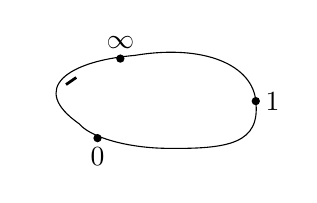
\begin{tikzpicture}[x=1cm,y=1cm]
\draw (0,0) .. controls (-.65,.45) and (-.15,.8) .. (.7,.87)
 .. controls (1.6,1.02) and (2.2,.74) .. (2.24,.29)
 .. controls (2.3,-.25) and (1.9,-.32) .. (1.1,-.31)
 .. controls (.55,-.3) and (.12,-.15) .. (0,0);
\draw[line width=1pt] (-.17,.5) -- (-.04,.59);
\fill (.52,.83) circle (1.5pt) node[above] {$\infty$};
\fill (2.24,.29) circle (1.5pt) node[right] {$1$};
\fill (.23,-.18) circle (1.5pt) node[below] {$0$};
\end{tikzpicture}}
\diagram{\begin{tikzcd}[ampersand replacement=\&,column sep=large]
1 \arrow[r] \& \mu_\nu(\overline{\mathbb Q}) \arrow[r] \& \Gamma'_{\deleted{\unsure{n}}} \arrow[r] \& (\mathbb Z/n\mathbb Z)^* \arrow[r] \& 1
\end{tikzcd}}
$\nu=\text{ordre de }2\text{ dans }\deleted{\unsure{\mathbb Q^*}}\ K_n^*/K_n^{*n}$, où $K_n=\mathbb Q(\sqrt[n]{1})$.
\[
\begin{array}{rcll}
0,1,\infty&\longmapsto&0&\text{ordre }2\\
\tfrac12,2,-1&\longmapsto&1&\text{ordre }2\\
-j,-\bar j&\longmapsto&\infty&\text{ordre }3
\end{array}
\]
\par\noindent\rule{.7\linewidth}{.2pt}
\[
g(z)=\frac{27z^2(z-1)^2}{4(z^2-z+1)^3}\qquad
 gf(z)=\frac{27}{4}\frac{z^{2n}(z^n-1)^2}{(z^{2n}-z^n+1)^3}
\]
\[\lambda\frac4{27}=1\]
\[
g(z)=1\Longleftrightarrow
\underbrace{4(z^2-z+1)^3-27z^2(z-1)^2}_{\begin{aligned}
&\unsure{-4|4}\bigl[(z+1)(z-\tfrac12)(z-2)\bigr]^2
=4\bigl[(z+1)(z^2-\tfrac52+1)\bigr]^2\\
&\hspace{6em}=\bigl[(z+1)(2z^2-5+2)\bigr]^2
\end{aligned}}=0
\]
% Dans les deux derniers facteurs, aucun z distinct n'est visible après 5/2 ni après 5 ; aucune correction algébrique n'est introduite.

\scanpage{20}
% Foliotation archivistique au crayon, en bas à gauche : 19.
\diagram{\begin{tikzcd}[ampersand replacement=\&,column sep=small,row sep=large]
D \arrow[r,phantom,"\subset"] \arrow[d,"\text{fini}"'] \& \mathbb G_m \arrow[dl,no head] \\
\mathbb Q \&
\end{tikzcd}}
\diagram{\begin{tikzcd}[ampersand replacement=\&,row sep=large,column sep=small]
\& \vdots \& \\
\& {}_{\unsure{n}}U \arrow[d,no head] \& \\
\underline{\operatorname{Hom}}(D,\mathbb G_m) \arrow[d,"n"] \arrow[r,phantom,"="] \& U \arrow[d,"n"] \& \xi \\
\underline{\operatorname{Hom}}(D,\mathbb G_m) \arrow[r,phantom,"="] \& U \arrow[d,no head] \& \\
\& \vdots \&
\end{tikzcd}}
\[T(\mathbb Q)\ni\xi\qquad H^1(\mathbb Q,T_\infty(U))\]
\figure{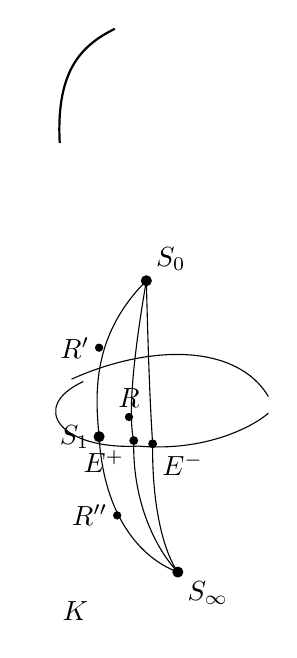
\begin{tikzpicture}[x=1cm,y=1cm]
\draw[line width=.8pt] (-.9,3.25) .. controls (-.95,4.2) and (-.6,4.5) .. (-.2,4.7);
\draw (-.6,.22) .. controls (-1.3,-.1) and (-.9,-.65) .. (.1,-.6)
 .. controls (1.05,-.68) and (1.65,-.28) .. (1.75,-.18);
\draw (-.75,.25) .. controls (.25,.7) and (1.35,.7) .. (1.75,.03);
\draw (.2,1.5) .. controls (-.5,.8) and (-.45,.05) .. (-.4,-.48)
 .. controls (-.34,-1.48) and (.12,-2.02) .. (.6,-2.2);
\draw (.2,1.5) .. controls (.02,.45) and (-.03,-.22) .. (.04,-.53)
 .. controls (.02,-1.35) and (.35,-1.94) .. (.6,-2.2);
\draw (.2,1.5) .. controls (.22,.72) and (.24,.04) .. (.28,-.57)
 .. controls (.27,-1.45) and (.45,-1.99) .. (.6,-2.2);
\fill (.2,1.5) circle (2pt) node[above right] {$S_0$};
\fill (-.4,-.48) circle (2pt) node[left] {$S_1$};
\fill (.6,-2.2) circle (2pt) node[below right] {$S_\infty$};
\fill (-.4,.65) circle (1.5pt) node[left] {$R'$};
\fill (-.17,-1.48) circle (1.5pt) node[left] {$R''$};
\fill (.04,-.53) circle (1.6pt) node[below left] {$E^+$};
\fill (.28,-.57) circle (1.6pt) node[below right] {$E^-$};
\fill (-.02,-.23) circle (1.5pt) node[above] {$R$};
\node at (-.7,-2.7) {$K$};
\end{tikzpicture}}
\diagram{\begin{tikzcd}[ampersand replacement=\&,column sep=huge,row sep=large]
\Gamma \arrow[r] \arrow[dr,"{\text{image de dim }\unsure{n+1|11+1}\ ?}"'] \& \operatorname{Aff}(T_\infty(U)) \arrow[d] \\
\& \operatorname{Aut}(T_\infty(U))
\end{tikzcd}}
Ss-grpe d'indice fini : opère par homothéties

$\unsure{\xi_i|\zeta_i}$ --- $\unsure{\mathbb Z}$-indép. mod racines de $1$
\diagram{\begin{tikzcd}[ampersand replacement=\&,column sep=large,row sep=large]
\Gamma \arrow[r] \arrow[dr] \& \operatorname{Aff}(n,\widehat{\mathbb Z}) \arrow[d] \\
\& \widehat{\mathbb Z}^{*}\cdot\widehat{\mathbb Z}^{n}
\end{tikzcd}}
\deleted{image de}
\margin{image d'indice fini ???}

\scanpage{21}
% Foliotation archivistique au crayon, en bas à gauche : 20.
\diagram{\begin{tikzcd}[ampersand replacement=\&]
\mathbb Q^* \arrow[r,no head] \& Z^1(\Gamma,\mathbb Z/n\mathbb Z)
\end{tikzcd}}
\deleted{$\unsure{\varphi(\xi)}$}
\[
\frac{\gamma\cdot\sqrt[n]{\xi}}{\sqrt[n]{\xi}}=1
\qquad
\gamma(\sqrt[n]{\xi})=\sqrt[n]{\unsure{\xi}}\quad\forall\gamma\in\Gamma
\]
\[\sqrt[n]{\xi}\in\mathbb Q\qquad\xi\in\mathbb Q^{*n}\]
\diagram{\begin{tikzcd}[ampersand replacement=\&,column sep=large,row sep=large]
\varprojlim\mathbb Q^*/\mathbb Q^{*n} \arrow[r] \& Z^1(\Gamma,\widehat{\mathbb Z}) \\
\& \widehat{\mathbb Z} \arrow[u] \\
\& 0 \arrow[u]
\end{tikzcd}}
\diagram{\begin{tikzcd}[ampersand replacement=\&,column sep=large,row sep=large]
\& 0 \\
\mathbb Q^*/\mathbb Q^{*n} \arrow[r,no head,"\sim"] \arrow[dr] \& H^1(\Gamma,\mathbb Z/n\mathbb Z) \arrow[u] \\
\mathbb Q^*/\mathbb Q^{*n}\oplus(\mathbb Z/n\mathbb Z)\ldots \arrow[r,phantom,"\simeq"] \& Z^1(\Gamma,\mathbb Z/n\mathbb Z) \arrow[u] \\
\& (\mathbb Z/n\mathbb Z)/\deleted{\substack{\text{éléments d'ordre }\unsure{2}\text{ de }\mathbb Z/n\mathbb Z\\\text{\unsure{fixés par un ss-grpe}}\\\text{de}}} \arrow[u] \\
\& 0 \arrow[u]
\end{tikzcd}}
\[
\mathbb Z/2^n\mathbb Z
\]
$a=na$ si $n$ impair
\[2a=0\]
\diagram{\fbox{$\begin{tikzcd}[ampersand replacement=\&]
\Gamma \arrow[r] \& \operatorname{Aff}(1,\widehat{\mathbb Z})
\end{tikzcd}$}}
\deleted{$\unsure{Z}$}
\[
Z^1(\Gamma,\widehat{\mathbb Z})\simeq
\underbrace{\varprojlim\mathbb Q^*/\unsure{\mathbb Q^{*n}}}_{\displaystyle\{\pm1\}+\underbrace{\varprojlim(\mathbb Z/n\mathbb Z)^P}_{\widehat{\mathbb Z}^{P}}}
\oplus\widehat{\mathbb Z}
\]
$K_{\unsure{c|\ell}\infty}$ corps cyclotomique
\[K_{\unsure{c|\ell}\infty}^{*}/\mathbb Q^{*}\]

\scanpage{22}
% Foliotation archivistique au crayon, en bas à gauche : 21.
\deleted{$\unsure{\widehat{\mathbb Z}^{*}}$}

$\Gamma$ opère sur $\bar X'_\xi$\qquad ($\unsure{\eta|\xi}\in\mathbb Q_+^*$)

\inserted{$\unsure{\pi}$ opère trivialt}
\[
\unsure{\simeq}\ \bar X'_{-1}\qquad
\bigl[\bar X'_{(-1)^\epsilon}\wedge\bar X'_{|\xi|}
\]
\[\exp\frac{2i\pi}{2n}=\exp\frac{i\pi}{n}\]
\diagram{\begin{tikzcd}[ampersand replacement=\&,column sep=large,row sep=large]
\mathbb Q^* \arrow[r] \arrow[d,phantom,"\simeq",sloped] \& \deleted{\operatorname{Hom}(\unsure{\Gamma}}\ Z^1(\Gamma,\widehat{\mathbb Z}^{*}) \arrow[r] \& H^1(\Gamma,\widehat{\mathbb Z}) \\
\unsure{\mathbb Z/2\mathbb Z|\mathbb Z/n\mathbb Z}\oplus\mathbb Z^{(P)} \& \&
\end{tikzcd}}
\[\mathbb Z[\]
\[\varphi(\gamma\gamma')=\varphi(\gamma)+\gamma\varphi(\gamma')\]
\deleted{$\unsure{a-\varphi(\gamma)}$}
\[\varphi(\gamma)=a-\gamma a\]
\diagram{\begin{tikzcd}[ampersand replacement=\&]
\mathbb Q^* \arrow[r] \& Z^1(\Gamma,\widehat{\mathbb Z}_\ell)
\end{tikzcd}}
\deleted{$\mathbb Q^*/\mathbb Q^{*\unsure{\ell^n|\ell^\infty}}$}
\deleted{$\mathbb Z_\ell^P$}
\diagram{\begin{tikzcd}[ampersand replacement=\&]
\widehat{\mathbb Z}^{\unsure{P|n}} \arrow[r] \& Z^1
\end{tikzcd}}
\[\varprojlim_n Z^1(\Gamma,\mathbb Z/n\mathbb Z)\]
\[
\begin{aligned}
\mathbb Q^*/\mathbb Q^{*n}&\simeq H^1(\Gamma_{\unsure{k|K}},\mu_n)\\
&\simeq Z^1(\unsure{\overline{\mathbb Q}|\Gamma},\mathbb Z/n\mathbb Z)
\end{aligned}
\]
\figure{\begin{tikzpicture}
\draw (0,1.7) .. controls (1,.9) and (1.1,1.3) .. (1.6,.6) -- (2.1,-.4);
\draw (2.15,-.5) -- (3.7,-.85);
\end{tikzpicture}}
\deleted{$a\in\mathbb Q^*\qquad\overline{\mathbb Q}$}
\[
(a,\overset{\deleted{\unsure{a}}}{\xi})\in\overline{\mathbb Q}
\qquad \xi^n\in\mathbb Q^*
\]
\deleted{$\unsure{-a}$}
\[\sqrt[n]{p_1}-\sqrt[n]{p_\nu}\]
\[\mathbb Q^*\subset\overline{\mathbb Q}^{*}\qquad {}_n(\overline{\mathbb Q}^{*}/\mathbb Q^*)\]
\[K=K_{A,\unsure{n}}=\mathbb Q(\sqrt[n]{p_1},\,-\,,\sqrt[n]{p_\nu})\]
\[\Pi\qquad K^*/\mathbb Q^*\]

\scanpage{23}
% Foliotation archivistique au crayon, en bas à gauche : 22.
\diagram{\begin{tikzcd}[ampersand replacement=\&,row sep=large,column sep=large]
\mathbb G_{m\,\mathbb Q} \arrow[d,"{\lambda\mapsto\lambda^n}"] \& \\
\mathbb G_{m\,\mathbb Q} \arrow[d,no head] \& \\
\mathbb Q \arrow[r,no head] \& \overline{\mathbb Q}
\end{tikzcd}}
\diagram{\begin{tikzcd}[ampersand replacement=\&]
1 \arrow[r] \& \mu_n \arrow[r,no head] \& \mathcal E'_n \arrow[r,no head] \& \Gamma' \arrow[l,bend left=25] \arrow[r] \& 1
\end{tikzcd}}
\[
\mathcal E'_n=\underbrace{\bigl[(\mathbb Z/6n\mathbb Z)^*\cdot\mu_\nu\bigr]}_{\downarrow\,\operatorname{Aff}(\mu_{\unsure{n|\nu}})}\cdot\mu_n
\]
\deleted{$\Gamma'\simeq(\mathbb Z/6n\mathbb Z)^*\cdot\mu_\nu$}
\diagram{\begin{tikzcd}[ampersand replacement=\&,column sep=large,row sep=huge]
1 \arrow[r] \& \mu_\nu \arrow[r] \& \Gamma'_\nu \arrow[r,no head] \& (\mathbb Z/\nu\mathbb Z)^* \arrow[r,no head] \& 1 \\
1 \arrow[r] \& \mu_\nu \arrow[u,equal] \arrow[r] \& \Gamma'_{\unsure{\xi|n}} \arrow[u] \arrow[r,no head] \& (\mathbb Z/6n)^* \arrow[u] \arrow[r] \& 1
\end{tikzcd}}
\margin{\unsure{splitté|splitte}, splitting dépend du choix de $\sqrt[\nu]{2}$ sur $K_\nu$.}
\[
\left.
\begin{array}{ccccc}
E^+&R'&R&S_1&S_0\ \deleted{\unsure{S_\infty}}\\
\wr&\wr&\wr&\wr&\wr\\
E^-&R''&R&S_1&\unsure{S_2|S_\infty}
\end{array}
\right\}\quad r\quad z\mapsto\frac1z
\]
\diagram{\begin{tikzcd}[ampersand replacement=\&,column sep=large]
1 \arrow[r] \& T_\infty(\overline{\mathbb Q}) \arrow[r,no head] \& \mathcal E_\infty \arrow[r,no head] \& \Gamma \arrow[r] \& 1
\end{tikzcd}}
\[
\Gamma\cdot\underbrace{T_\infty(\overline{\mathbb Q})}_{T_\infty\ (\underset{\text{\unsure{non-can}}}{\simeq}\widehat{\mathbb Z})}
\]
$\Gamma$ opère via $\widehat{\mathbb Z}^{*}$

\deleted{$\unsure{\widehat{\mathbb Z}},\ R',R'',1$}

$E^+,E^-,R,R',R'',S_1$ sont torseurs sous $\mu_\infty$

\deleted{$E^+\simeq(E^-)^\vee,\quad R'\simeq$}
\[
E^+\wedge E^-=1,\quad R'\wedge R''=1,\quad R^2=1.
\]
\[E^{+\,6}=1\]

\scanpage{25}
\uline{1.1} Soit $n\in\mathbb N^*$, et posons
$C_n\subset\mathbb P^2_{\mathbb Q}$ équation projective
\[
(1)\qquad x^n+y^n+z^n=0
\]
Le groupe $\mu_{n\mathbb Q}^3$ opère sur $\mathbb E^3_{\mathbb Q}$ par matrices diagonales,
donc posant
\[
(2)\qquad \Pi_{n\mathbb Q}=\mu_n^3/\underset{\substack{\curvearrowright\,\text{diag.}}}{\mu_n}
\simeq\mu_n\otimes_{\mathbb Z}(\mathbb Z^3/\mathbb Z)
\]
\margin{NB on écrit $\mu_n$ au lieu de $\mu_{n\mathbb Q}$}
opère sur $\mathbb P^2_{\mathbb Q}$, en laissant $C_n$ invariant. La courbe
$C_n/\Pi_{n\mathbb Q}$ s'identifie à la courbe \inserted{$C_1$} qui est donnée,
en coordonnées homogènes, par
\[
(3)\qquad X+Y+Z=0
\]
\margin{Comme carte pondérée, elle est formée de $2n^2$ triangles
ch. sommet est d'ordre $2n$, chaque type de sommet \unsure{intervient} $n$ fois\ldots}
qu'on identifie à $\mathbb P^1_{\unsure{x}}$, en envoyant les points de $C_1$
pour lesquels $X,Y$ ou $Z$ sont nuls resp. en $0,1,\infty$.
Donc écrivant $C_1$ en coordonnées affines, faisant $Z=1$
i.e. $X/Z=\xi$, $Y/Z=\eta$, sous la forme
\[
(3')\qquad \xi+\eta+1=0
\]
i.e.
\[
\eta=-1-\xi
\]
$\xi=0$ correspond à $\eta=-1$, $\eta=0$ à $\xi=-1$, donc posant
\[
(3'')\qquad t=-\xi\qquad\text{donc}\quad \xi=-t,\ \eta=t-1,\ \zeta=1
\]
les valeurs de $t$ pour lesquelles $X=0$, $Y=0$, $Z=0$ sont resp. $t=0,1,\infty$.

\margin{Il y a en $\unsure{\alpha(i)|\alpha_i}$ $(i=0,1,\infty)$
$n$ p\textsuperscript{ts} de ramification de $C_n$, chacun de degré de ramification $n$.}
$C_n$ est étale sur $C_1=\mathbb P^1_{\mathbb Q}$ sauf en $0,1,\infty$, \unsure{un|on}
\unsure{donne|trouve} rev. principal $C_n^*$ de $C_1^*\simeq\mathbb P^1_{\mathbb Q}\setminus\{0,1,\infty\}$,
groupe $\Pi_{n\mathbb Q}$.
% archive foliation: 24

\scanpage{26}
1.2. Les $C_n$ forment un syst. projectif de $\mathbb Q$-schémas.
\diagram{\[
(4)\qquad\begin{tikzcd}[ampersand replacement=\&,column sep=large]
C_{n'}\arrow[r]\&C_n\\
(X^d,Y^d,\unsure{Z}^d)\&X,Y,Z\arrow[l]
\end{tikzcd}
\qquad\text{si }n\mid n'\quad\text{soit }n'=nd
\]}
morphismes compatibles avec les
\diagram{\[
(4')\qquad\begin{tikzcd}[ampersand replacement=\&]\Pi_{n'}\arrow[r]\&\Pi_n\end{tikzcd}
\]}
\margin{\uline{NB} on laisse tomber l'indice $\mathbb Q$}
déduits des hom. canoniques
\diagram{\[
(4'')\qquad\begin{tikzcd}[ampersand replacement=\&]\mu_{n'}\arrow[r]\&\mu_n\end{tikzcd}
\]}
Passant à la limite, on trouve
\[
(5)\qquad\left\{\begin{aligned}
C_\infty&=\varprojlim_n C_n\\
C_\infty^*&=\varprojlim_n C_n^*
\end{aligned}\right.
\]
sur lequel opère
\[
\begin{aligned}
(6)\qquad\Pi_\infty&=\varprojlim_n\Pi_n
\simeq\deleted{\unsure{\widehat{\mathbb Z}}}\, .\,\overleftarrow{\mu}_\infty
\otimes_{\unsure{\widehat{\mathbb Z}|\mathbb Z}}(\mathbb Z^3/\mathbb Z)\\
&\simeq\overleftarrow{\mu}_\infty\otimes_{\widehat{\mathbb Z}}
(\widehat{\mathbb Z}^{\,3}/\widehat{\mathbb Z})
\end{aligned}
\]
où
\[
\overleftarrow{\mu}_\infty=\varprojlim_n\mu_n
\]
Ainsi $C_\infty^*$ devient rev. principal de $C_1^*$, de groupe $\Pi_\infty$.
% archive foliation: 25

\scanpage{27}
1.3. Notons que $\unsure{\mathfrak S_3|\mathbb G_3}$ opère sur $C_n$ de façon évidente,
et les $C_{n'}\longrightarrow C_n$ sont des $\unsure{\mathfrak S_3|\mathbb G_3}$-morphismes,
donc $\unsure{\mathfrak S_3|\mathbb G_3}$ opère sur $C_\infty$.
L'opération de $\unsure{\mathfrak S_3|\mathbb G_3}$ sur $C_1$ \inserted{$\simeq\mathbb P^1_{\mathbb Q}$}
est celle déduite des opérations de $\unsure{\mathfrak S_3|\mathbb G_3}$ sur $\{0,1,\infty\}$.
\inserted{Enfin, $\unsure{\mathfrak S_3|\mathbb G_3}$ opère sur $\Pi_n$, de façon que
$\unsure{\mathfrak S_3|\mathbb G_3}$ opère sur $(C_n,\Pi_n\ldots)$ -- donc
$\unsure{\mathfrak S_n|\mathfrak S_3}$ opère sur $(C_\infty,\Pi_\infty)\ldots$}

1.4. Considérons la clôture alg. $\overline{\mathbb Q}$ de $\mathbb Q$ dans $\mathbb C$,
d'où par changement de base des schémas $\overline C_n$, $\overline C_n^*$,
$\overline C_\infty$, $\overline C_\infty^*$ sur $\overline C_1=\mathbb P^1_{\overline{\mathbb Q}}$
et $\overline C_1^*=\mathbb P^1_{\overline{\mathbb Q}}\setminus\{0,1,\infty\}$.
Sur ces schémas $C_n$
\deleted{$\unsure{\Gamma=\operatorname{Gal}}$}
\[
(7)\qquad\Gamma=\operatorname{Gal}(\overline{\mathbb Q}/\mathbb Q)
\]
opère de façon évidente, et \unsure{ajoutant|adjoignant} les groupes
\[
(8)\qquad\left\{\begin{aligned}
&\inserted{\pi_n=}\deleted{\unsure{\Gamma}}\,
\Pi_n(\overline{\mathbb Q})=
\unsure{\overline\mu_n^{\,3}|\mu_n^3}/\unsure{\overline\mu_n|\mu_n}
\simeq\unsure{\overline\mu_n|\mu_n}\otimes_{\mathbb Z}\mathbb Z^3/\mathbb Z\\
&\hspace{4cm}\simeq\unsure{\overline\mu_n|\mu_n}\otimes_{\widehat{\mathbb Z}}
(\widehat{\mathbb Z}^{\,3}/\widehat{\mathbb Z})\\
&\text{où}\quad\inserted{\mu_n=\mu_n(\overline{\mathbb Q})}\\
&\qquad\deleted{\unsure{\overleftarrow\mu_\infty|\Pi_\infty}(\overline{\mathbb Q})=
\varprojlim_n\mu_n(\overline{\mathbb Q})}
\end{aligned}\right.
\]
et $\unsure{\mathfrak S_3|\mathbb G_3}$. On voit tout de suite que ces opérations
s'ajustent de façon à ce qu'opère sur ces courbes le groupe
\[
(\unsure{9|8})\qquad\mathcal E_n=
(\unsure{\mathfrak S_3|\mathbb G_3}\times\Gamma)
\mathbin{\underset{\scriptscriptstyle 1/2}{.}}\pi_n
\]
% archive foliation: 26

\scanpage{28}
où $\unsure{\mathfrak S_3|\mathbb G_3}\times\Gamma$ opère sur $\pi_n$
via l'opération évidente de $\unsure{\mathfrak S_3|\mathbb G_3}$ sur
$\mathbb Z^3/\mathbb Z$, et de $\Gamma$ sur $\mu_n$, via le caractère fondamental
\diagram{\[
(10)\qquad\begin{tikzcd}[ampersand replacement=\&]\Gamma\arrow[r,no head,"\chi_n"]\&(\mathbb Z/n\mathbb Z)^*\end{tikzcd}
\]}
Passant à la limite, on trouve une opération de
$\unsure{\mathfrak S_3|\mathbb G_3}\times\Gamma$ sur
\[
(11)\qquad\left\{\begin{aligned}
\pi_\infty&=T^3/T\simeq T\otimes\mathbb Z^3/\mathbb Z\\
&\simeq T\otimes\widehat{\mathbb Z}^{\,3}/\widehat{\mathbb Z}\\
\text{où}\quad T&=\varprojlim\mu_n=\overleftarrow\mu_\infty(\overline{\mathbb Q})
\end{aligned}\right.
\]
où $\unsure{\mathfrak S_3|\mathbb G_3}$ opère via son op. sur $\mathbb Z^3$ ou
$\widehat{\mathbb Z}^{\,3}$, et $\Gamma$ par le caractère fondamental
\diagram{\[
(12)\qquad\begin{tikzcd}[ampersand replacement=\&]\Gamma\arrow[r,"\chi_\infty=\chi"]\&\widehat{\mathbb Z}^{\,*}\end{tikzcd}
\]}
Bien entendu,
\[
(13)\qquad\left\{\begin{aligned}
\unsure{\mathfrak S_3|\mathbb G_3}\times\Gamma&=\operatorname{Aut}_{\mathbb Q}C_1\\
(\unsure{\mathfrak S_3|\mathbb G_3}\times\Gamma)
\mathbin{\underset{\scriptscriptstyle1/2}{.}}\mu_n
&\overset{\mathrm{dfn}}=\mathcal E_n=\operatorname{Aut}_{\mathbb Q}(C_n)\\
(\unsure{\mathfrak S_3|\mathbb G_3}\times\Gamma)
\mathbin{\underset{\scriptscriptstyle1/2}{.}}\mu_\infty
&\overset{\mathrm{dfn}}=\mathcal E_\infty=\operatorname{Aut}_{\mathbb Q}(C_\infty)
\end{aligned}\right.
\]

1.5. En fait, l'hom ext.
\diagram{\[
\begin{tikzcd}[ampersand replacement=\&,column sep=large,row sep=large]
\pi_1(\overline C_1^*)\arrow[r]\arrow[d,equal]\&
\pi_\infty\,\unsure{\sim}\arrow[d,phantom,"\unsure{\wr}"]\\
\pi_1(\mathbb P^1_{\overline{\mathbb Q}}\setminus\{0,1,\infty\})\&
T^3/T\simeq T\otimes\mathbb Z^3/\mathbb Z
\end{tikzcd}
\]}
définit un isom
% archive foliation: 27

\scanpage{29}
\diagram{\[
(14)\qquad\begin{tikzcd}[ampersand replacement=\&,row sep=large]
\pi_1(\overline C_1^*)_{\mathrm{ab}}\arrow[r,no head,"\sim"]\arrow[d,phantom,"\wr"]\&\pi_\infty\\
H_1(\overline C_1^*)\&
\end{tikzcd}
\]}
(i.e. on est en train de faire l'étude arithmétique des rev.
\inserted{étales} \uline{abéliens} de $\overline C_1^*\ldots$).

1.6. Considérons les fibres
\[
(\overline C_\infty)_\zeta,\quad\zeta=0,1,\infty,\quad\text{soit }E_0,E_1,E_\infty
\]
Alors $E_0=\varprojlim_n E_0(n)$
\[
\begin{aligned}
E_0(n)&=\{\underbrace{(x,y,z)}_{\in\overline{\mathbb Q}^{\,3}}\mid x=0,\ y^n+z^n=0\}/\mu_n\\
&\simeq\{(y,z)\in\overline{\mathbb Q}^{\,2}\mid(\overline y/\overline z)^n=-1\}/\mu_n\\
&\simeq\{\unsure{\lambda}\in\overline{\mathbb Q}\mid\overline\lambda^{\,n}=-1\}\\
&\simeq\deleted{\unsure{\lambda\in\overline{\mathbb Q}}}\ \text{image inverse de }-1\in\mu_2\\
&\hspace{3cm}\text{par }\mu_{2n}\longrightarrow\mu_2
\end{aligned}
\]
donc
\[
(15)\qquad\left\{\begin{aligned}
E_\zeta\overset{\varphi_\zeta}{\simeq}\ &\text{à l'image inverse de }-1\in\mu_2\text{ par}\\
&\unsure{\mu|T}\longrightarrow\mu_2
\end{aligned}\right.
\]
\inserted{Cet isom (pour $\zeta=0,1$ ou $\infty$ fixé) est compatible}
\deleted{De façon plus \unsure{intr.}}
avec l'action de \deleted{$\unsure{\Pi_\infty|\mathfrak S_3}$} $\Gamma$;
\deleted{et avec celle de $\pi_\infty$, opérant sur le deuxième m\textsuperscript{b}
via \deleted{par} l'action de $T^3/\mathrm{pr}_\zeta T\oplus\operatorname{diag}(T)$}
\inserted{Pour formuler} de façon simple des compatibilités avec les actions de
$\unsure{\mathfrak S_3|\mathbb G_3}$ et $\pi_\infty$, on va \unsure{présenter|procéder}
% archive foliation: 28

\scanpage{30}
les choses de façon plus intrinsèque. Considérons l'homomorphisme canonique
\diagram{\[
(16)\qquad\begin{tikzcd}[ampersand replacement=\&]\pi_\infty\arrow[r]\&\pi_2\end{tikzcd}
\]}
et soit
\[
(17)\qquad\pi_2^*=\pi_2\setminus\{1\}\simeq
\deleted{\unsure{(\mathbb Z/2\mathbb Z)^3/\mathbb Z/2\mathbb Z}}
\inserted{(\mathbb F_2^3/\mathbb F_2)\setminus\{0\}}
\]
c'est isom à l'ens $I=\{0,1,\infty\}$ de façon compatible avec l'action de
$\unsure{\mathfrak S_3|\mathbb G_3}$ [NB $\Gamma$ opère trivialt sur $\pi_2^*$
comme sur \inserted{$I=$} $\{0,1,\infty\}$]

Ceci dit, \deleted{\unsure{on a, et}}
\deleted{\[
(18)\qquad I=\{0,1,\infty\},\quad E(I)=\overline C_\infty(\overline{\mathbb Q})\mid I
=\coprod_{\zeta\in I}\overline C_{\infty\zeta}=E_0\amalg E_1\amalg E_\infty
\]
Posant $\widehat\mu_\infty=\mu_\infty\amalg\{0\}$
\[
(19)\qquad E(I)=\{(\zeta_0,\zeta_1,\zeta_\infty)\in\widetilde\mu_\infty^{\,3}
\mid\text{un des }\zeta_i\text{ est nul}\}
\]}
considérons la suite \deleted{\unsure{suivante|exacte} $\mu_\infty$}
\inserted{exacte de $(\unsure{\mathfrak S_3|\mathbb G_3}\times\Gamma)$-modules}
\diagram{\[
(18)\qquad\begin{tikzcd}[ampersand replacement=\&,column sep=large]
\unsure{0}\arrow[r]\&\pi_\infty\arrow[r,"2"]\&\pi_\infty\arrow[r,"p"]\&
\pi_2\arrow[r]\arrow[d,phantom,"\cup"]\&{}\\
\&\&\&I=\{0,1,\infty\}\&
\end{tikzcd}
\]}
et pour $i\in I$, soit \deleted{$\unsure{Z_i}$}
\diagram{\[
(19)\qquad\begin{tikzcd}[ampersand replacement=\&]
Z_i\arrow[r,phantom,"\subset"]\arrow[d,phantom,"\wr"]\&\pi_\infty\\
T\&
\end{tikzcd}
\]}
les \uline{ss-grpes de ramification} correspondants,
\margin{Autre façon on utilise les trois points rat/$\mathbb Q$ de
$\unsure{\overline C_\infty|\overline C_2}$, \deleted{\unsure{désignés}}
dans $E_i$ $(i=0,1,\infty)$ d'où $E_i\simeq\pi_\infty/Z_i
\simeq T\mathop{\wedge}_{(\pm1)}(I\setminus\{i\})$}
\unsure{images|image} dans $\pi_\infty\simeq T^3/T$ des \deleted{\unsure{hom.}}
facteurs $T$ d'indice $i$ dans $T^3$. \deleted{Soit enfin} On a donc
\[
(20)\qquad E_i\simeq p^{-1}(\{i\})/Z_i
\]
% archive foliation: 29

\scanpage{31}
1.7. Soient
\[
(21)\qquad(\alpha=-\overline j,\ \overline\alpha=-j)
\]
\margin{\uline{NB} $j=-\frac12+i\frac{\sqrt3}{2}$\quad
$-\overline j=\frac12+i\frac{\sqrt3}{2}$.
Posons $\alpha_{\unsure{*|2}}=\{\alpha,\overline\alpha\}$,
$E(\alpha_{\unsure{*|2}})=E(\{\alpha,\overline\alpha\})$}
les deux p\textsuperscript{ts} de $\overline C_1$ invariants par
$\unsure{\mathfrak S_3^+|\mathbb G_3^+}$ i.e. dont les orbites sous
$\unsure{\mathfrak S_3|\mathbb G_3}$ sont de card. $2$. On veut déterminer
\[
(22)\qquad E(\alpha)\amalg E(\overline\alpha)
\]
l'image inverse de $\{\alpha,\overline\alpha\}$ en tant que $\mathcal E$-ensemble
-- i.e. avec les op. de $\Gamma$, $\unsure{\mathfrak S_3|\mathbb G_3}$, $\pi_\infty$.
On trouve, par calcul en coordonnées affines
\[
(23)\qquad\left\{\begin{aligned}
E(\alpha)_n\deleted{\unsure{(\overline{\mathbb Q})}}&=
\{(\zeta,\eta)\in\overline{\mathbb Q}^{\,2}\mid\zeta^n=\overline j,\
\eta^n=\deleted{\unsure{-1-\overline j|-\overline j-1}}\ \inserted{\text{i.e.}}=j\}\\
E(\overline\alpha)_n\deleted{\unsure{(\overline{\mathbb Q})}}&=
\{(\unsure{\zeta},\eta)\in\overline{\mathbb Q}^{\,2}\mid\zeta^n=j,\ \eta^n=\overline j\}
\end{aligned}\right.
\]
\deleted{Notons qu'avec les conditions on aura
\[
\zeta^{3n}=\eta^{3n}=1
\]
donc
\diagram{\[
\begin{tikzcd}[ampersand replacement=\&,column sep=large]
E(\alpha)=\varprojlim E(\alpha)_n\&
\varprojlim\mu_{3n}\times\mu_{3n}\simeq\mu_\infty\times\mu_\infty\arrow[l]\\
(\zeta_n,\eta_n)\arrow[r,maps to]\&(\zeta_n^3,\eta_n^3)
\end{tikzcd}
\]}}
Pour avoir une description intrinsèque des opérations de
$\unsure{\mathfrak S_3|\mathbb G_3}$ et de $\pi_n$ (celles de $\Gamma$ sont
visibles sur la forme donnée) on va \deleted{\unsure{écrire}}
\deleted{plutôt} passer aux cônes affines projetants de $C_n$, $C_1$,
\deleted{et prendre les points au dessus des p\textsuperscript{ts} de
$E_n(\{\alpha,\overline\alpha\})_{\unsure{n}}$, $E_1(\{\alpha,\overline\alpha\})$,
\deleted{$\unsure{\mathbb Q}$}
\diagram{\[\begin{tikzcd}[ampersand replacement=\&]E_1(\alpha,\overline\alpha)\arrow[r]\&{}\end{tikzcd}\]}
disons $\widetilde E_n(\{\alpha,\overline\alpha\})$,
$\widetilde E_1(\{\alpha,\overline\alpha\})$ -- puis en
passer en quotient pour avoir $E_n$, $E_1\ldots$}
% archive foliation: 30

\scanpage{32}
\deleted{$\widetilde E_1\{\alpha,\unsure{\overline\alpha}$}
Soit
\deleted{\[
\widetilde C_1=\{(\zeta_1,\zeta_2,\zeta_\infty)\in\mu_3^3
\]}
\[
\begin{aligned}
(24)\qquad\widetilde C_1&\simeq\operatorname{Isom}(\underbrace{\{1,2,\unsure{\infty|3}\}}_I,\mu_3)\\
&\simeq\{(\zeta_1,\zeta_2,\zeta_3)\in\mu_3^3\mid
\zeta_1\ne\zeta_2\ne\zeta_3\ne\zeta_1\}\\
&\subset\deleted{\unsure{\mathbb E^3|\overline{\mathbb Q}^{\,3}}}\
\text{cône projetant de }\overline C_1\subset\overline{\mathbb Q}^{\,3}
\end{aligned}
\]
$\widetilde C_1$ a $3!=6$ éléments, et $\mu_3$ y opère diagonalement
\inserted{librement (\unsure{multiplication scalaire|multiplications scalaires})}
\deleted{sans point fixe} -- le quotient $\widetilde C_1/\mu_3$ a donc deux éléments.
L'application
\diagram{\[\begin{tikzcd}[ampersand replacement=\&]\widetilde C_1/\mu_3\arrow[r]\&\overline C_1\end{tikzcd}\]}
\margin{\uline{NB} $\widetilde C_1/\mu_3\subset\pi_3$ est formé des \deleted{\unsure{élém.}}}
induit une bijection
\[
(25)\qquad\widetilde C_1/\mu_3\simeq
\overline C_1^{\unsure{\mathfrak S_3^+|\mathbb G_3^+}}=\{\alpha,\overline\alpha\}
\]
mettant en évidence l'opération de $\mathcal E$ sur $(\alpha,\overline\alpha)$,
via son opération sur $\widetilde C_1\subset\mu_3^3=\mu_3^I$
[\uline{NB} $\mathcal E$ opère via $\unsure{\mathfrak S_3|\mathbb G_3}\times\{\pm1\}$,
avec $\Gamma\overset{\chi_3}{\longrightarrow}\{\pm1\}$)

Soit alors $\widetilde C_n$ l'image inverse de $\widetilde C_1$ par
l'application $\cdot^n$ du cône projetant de $\overline C_n$, au cône projetant
de $\overline C_1$, donc c'est
\deleted{l'ens des $(x,y,z)$ \unsure{sur} $\unsure{E_n}$}
\[
(26)\qquad\left\{\begin{aligned}
\overline C_n&=\{(x,y,z)\in\overline{\mathbb Q}^{\,3}\mid
\deleted{x^n+y^n+z^n=1,\ x}\
\inserted{(x^n,y^n,z^n)\in\widetilde C_1}\}\\
&=\{(x,y,z)\in\overline{\mathbb Q}^{\,3}\mid
x^{3n}=y^{\unsure{2n|3n}}=z^{3n}=1,\
x^{\unsure{2n|n}}\ne y^n\ne z^n\ne x^n\}
\end{aligned}\right.
\]
Noter que $\mu_{3n}$ opère diagonalement sur $\overline C_n$,
% archive foliation: 31

\scanpage{33}
L'application
\diagram{\[\begin{tikzcd}[ampersand replacement=\&]\widetilde C_n\arrow[r]\&\widetilde C_1\end{tikzcd}\]}
est compatible avec
\diagram{\[\begin{tikzcd}[ampersand replacement=\&]\mu_{3n}\arrow[r,"\zeta\mapsto\zeta^n"]\&\mu_3\end{tikzcd}\]}
et induit donc par passage au quotient
\diagram{\[\begin{tikzcd}[ampersand replacement=\&]\widetilde C_n/\mu_{3n}\arrow[r]\&
\widetilde C_1/\unsure{\mu_n|\mu_3}\end{tikzcd}\]}
Ceci dit, on a un diagramme comm.
\diagram{\[
(27)\qquad\begin{tikzcd}[ampersand replacement=\&,column sep=huge,row sep=large]
\widetilde C_n/\mu_{3n}\arrow[r]\arrow[d,"\wr"']\&
\widetilde C_1/\unsure{\mu_n|\mu_3}\arrow[d,phantom,"\wr"]\\
E_n(\underbrace{\{\alpha,\overline\alpha\}}_{\unsure{\alpha_*|\sigma_\alpha}})
\arrow[r,"\substack{\text{projection canonique}\\\text{induite par }\overline C_n\to\overline C_1}"']\&
E_1(\underbrace{\{\alpha,\overline\alpha\}}_{\unsure{\alpha_*|\sigma_\alpha}})
\end{tikzcd}
\]}
Passant à la limite, on pose
\[
(28)\qquad\widetilde C_\infty=
\{(x,y,z)\in T^3\,\unsure{\varphi|\mathrm{dfn}}=\mu_\infty^3
\mid x_3\ne y_3\ne z_3\ne x_3\}
\]
où pour $\zeta\in T$, $\zeta_3$ désigne son image dans $T/3T\simeq\mu_3$.
Donc $\unsure{\mathcal E_\zeta}$
\[
\widetilde C_\infty\subset T^3\qquad\text{stable par }T
\]
et on trouve une
\diagram{\[
(29)\qquad\begin{tikzcd}[ampersand replacement=\&,column sep=large]
\widetilde C_\infty/T\arrow[r,hook]\arrow[d,phantom,"\wr"]\&T^3/T\simeq\pi_\infty\\
E(\unsure{\alpha_*|\alpha}\deleted{\unsure{\overline\alpha}})\&
\end{tikzcd}
\]}
% archive foliation: 32

\scanpage{34}
de façon précise
\[
(30)\qquad\begin{aligned}
\widetilde C_\infty/\mu_\infty&\simeq\text{Image inverse de }
\overbrace{\overline C_1/\mu_3}^{\substack{\omega\\\wr}}
\subset\mu_3^3/\mu_3=\pi_3\\
&\hspace{2cm}\text{par }\pi_\infty\longrightarrow\pi_3
\end{aligned}
\]
En vertu de la suite exacte
\diagram{\[
(31)\qquad\begin{tikzcd}[ampersand replacement=\&,column sep=large]
0\arrow[r,no head]\&\pi_\infty\arrow[r,"3"]\&\pi_\infty\arrow[r,"p_3"]\&
\pi_3\arrow[r,no head]\arrow[d,phantom,"\cup"]\&0\\
\&\&\&\omega\&
\end{tikzcd}
\]}
$\pi_\infty$ opère librement sur cette partie de $\pi_\infty$, l'image inverse de
$\omega$ par $\pi_\infty\longrightarrow\pi_3$. Ceci donne les opérations de
$\pi_\infty$ sur $E(\alpha_*\deleted{\unsure{\overline\alpha}})\simeq p_3^{-1}(\omega)$,
celles de $\Gamma$ et $\unsure{\mathfrak S_3|\mathbb G_3}$ étant induites par
leurs opérations sur $\pi_\infty\ldots$.

\uline{NB} Sur $\pi_3$ \deleted{$\unsure{\mathcal E}\times$}
$\unsure{\mathfrak S_3|\mathbb G_3}\times\Gamma$ opère via
$\unsure{\mathfrak S_3|\mathbb G_3}\times\{\pm1\}$,
\margin{opère par homothéties sur $\pi_3$}
($\Gamma\overset{\chi_3}{\longrightarrow}\{\pm1\}$).
Considérons $\unsure{\mathfrak S_3^+|\mathbb G_3^+}$ \inserted{$\simeq\mathbb Z/3\mathbb Z$}
opérant sur $\pi_3$ $(\simeq\mathbb F_3^2)$, alors on sait qu'il doit y avoir
une droite invariante -- \deleted{\unsure{et les}} en fait elle est unique -- et
$\omega$ est formé des deux éléments non nuls de cette droite\ldots
% archive foliation: 33

\scanpage{35}
(1.8) Considérons enfin les p\textsuperscript{ts} fixes
\[
(32)\qquad\deleted{\unsure{\beta_0}}\inserted{\alpha'(0)}=2,\quad
\deleted{\unsure{\beta_1}}\inserted{\alpha'(1)}=-1,\quad
\deleted{\unsure{\beta_\infty}}\inserted{\alpha'(\infty)}=\frac12
\]
\figure{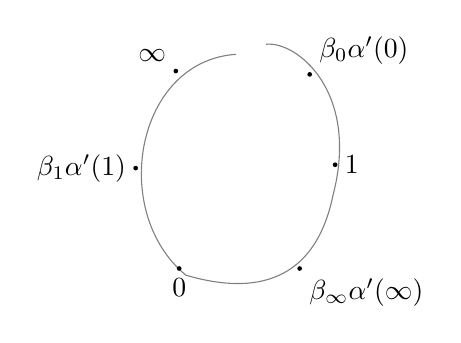
\begin{tikzpicture}[scale=.85]
\draw[gray] (0,1.65).. controls(-1.5,1.55) and(-1.9,-.7)..(-.75,-1.65)
.. controls(.1,-1.9) and(1.15,-1.9)..(1.45,-.45)
.. controls(1.85,1.1) and(.9,1.85)..(.45,1.8);
\foreach \x/\y in {-.9/1.4,1.1/1.35,1.48/0,.95/-1.55,-.85/-1.55,-1.5/-.05}
\fill (\x,\y) circle(.035);
\node[above left] at(-.9,1.4){$\infty$};
\node[above right] at(1.1,1.35){$\deleted{\unsure{\beta_0}}\inserted{\alpha'(0)}$};
\node[right] at(1.48,0){$1$};
\node[below right] at(.95,-1.55){$\deleted{\unsure{\beta_\infty}}\inserted{\alpha'(\infty)}$};
\node[below] at(-.85,-1.55){$0$};
\node[left] at(-1.5,-.05){$\deleted{\unsure{\beta_1}}\inserted{\alpha'(1)}$};
\end{tikzpicture}}
qui sont les p\textsuperscript{ts} fixes, autres que $0,1,\infty$ resp., des
transpositions $\tau_0$, $\tau_1$, $\tau_\infty\in\unsure{\mathfrak S_3|\mathbb G_3}$.
soit
\figure{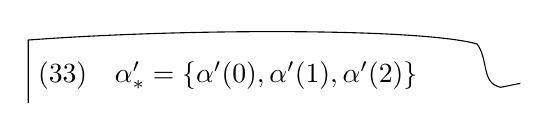
\begin{tikzpicture}
\node[anchor=west] at(0,0){$(33)\quad\alpha'_*=
\{\alpha'(0),\alpha'(1),\alpha'(2)\}$};
\draw (0,-.35)--(0,.45).. controls(2,.6) and(5,.6)..(5.7,.4)
.. controls(5.85,.2) and(5.75,-.1)..(6,-.15)--(6.25,-.1);
\end{tikzpicture}}
On veut déterminer $E(\alpha'_*)$ \inserted{$=\coprod_{i\in I}E(\alpha'(i))$}
comme $\mathcal E$-ensemble.
On trouve
\[
(34)\qquad\left\{\begin{aligned}
E_n(\alpha'(i))&\simeq\{(\zeta_j)\in\overline{\mathbb Q}^{\,I\setminus\{i\}}
\mid\zeta_j^{\unsure{n}}=-\tfrac12\quad\forall j\in I\setminus\{i\}\}\\
&\simeq K_n(-\tfrac12)^{I\setminus\{i\}}\\
E(\alpha'(i))&\simeq K(-\tfrac12)^{I\setminus\{i\}}
\end{aligned}\right.
\]
où $\forall\zeta_0\in\overline{\mathbb Q}$, on pose
\[
(35)\qquad\left\{\begin{aligned}
K_n(\unsure{\zeta|\varphi})&=\{\zeta\in\overline{\mathbb Q}\mid\zeta^n=\zeta_0\}\\
K_\infty(\zeta)=K(\zeta)&=\varprojlim_nK_n(\zeta)
\end{aligned}\right.
\]
$K_\infty(\zeta)$ étant un torseur sous $T=\mu_\infty$, sur lequel $\Gamma$ opère
donc un \deleted{$\unsure{\mathcal E}$} $(\mu_\infty,\Gamma)$-torseur\ldots)
Ici on \unsure{aura|a}, en vertu des rel. can.
\[
K(\unsure{\zeta\zeta'})\deleted{\unsure{=}}\simeq
K(\zeta)\mathbin{\wedge}_{T_\infty}K(\zeta')
\]
\[
(36)\qquad K(-\tfrac12)\simeq K(-1)\mathbin{\wedge}_T K(\tfrac12)
\simeq K(-1)\mathbin{\wedge}_T K(2)^{-1}
\]
\diagram{\[
(37)\qquad\begin{tikzcd}[ampersand replacement=\&]
\underbrace{K(-1)}_{\wr\ p_2^{-1}(\{\unsure{+1|-1}\})}\arrow[r,hook]\&
\deleted{\unsure{E_0}}\ T
\end{tikzcd}
\qquad
\left(\begin{tikzcd}[ampersand replacement=\&,column sep=small]
1\arrow[r]\&T\arrow[r,"2"]\&T\arrow[r,"p_2"]\&\mu_2\arrow[r]\&\unsure{1}
\end{tikzcd}\right)
\]}
% archive foliation: 34

\scanpage{36}
Soit
\[
(38)\qquad\unsure{A^*|A'}=\operatorname{Aff}(T,K(\tfrac12))\
\deleted{\unsure{\simeq\operatorname{Aff}}}
\]
donc
\diagram{\[
(39)\qquad\begin{tikzcd}[ampersand replacement=\&,column sep=large]
1\arrow[r]\&\deleted{\unsure{\mu_\infty}}\ T\arrow[r]\&A\arrow[r]\&
\widehat{\mathbb Z}^{\,*}\arrow[r,no head]\arrow[d,phantom,"\wr"]\&1\\
\&\&\&\operatorname{Aut}(T)\&
\end{tikzcd}
\]}
\deleted{Les ensembles \inserted{groupes $\mu_n,\mu_\infty=T$,}
$\pi_n,\pi_\infty$, et les ensembles $E_n(I)$, $E(I)$,
\unsure{Hom de} \illegible{2} \unsure{leurs}
$E_n(\alpha_*)$, $E(\alpha_*)$}
$A$ opère sur $\pi_n$, $\pi_\infty$ \inserted{$=T^3/T$}
par l'intermédiaire de $\widehat{\mathbb Z}^{\,*}$,
\deleted{\diagram{\[\begin{tikzcd}[ampersand replacement=\&]\Gamma\arrow[r]\&A\end{tikzcd}\]}}
(par homothéties scalaires\ldots) et le groupe
\[
\widetilde{\mathcal E}=(\unsure{\mathfrak S_3|\mathbb G_3}\times A)
\mathbin{\underset{\scriptscriptstyle1/2}{.}}\pi_\infty
\]
opère \inserted{de façon évidente} sur les ensembles
\inserted{$E_n(\unsure{\alpha(\infty)|\alpha(I)})$, $E(\unsure{\alpha(\infty)|\alpha(I)})$}
$E_n(\alpha_*)$, $E(\alpha_*)$, $E_n(\alpha'_*)$, $E(\alpha'_*)$
-- sur les quatre premiers il opère via le quotient
\deleted{$\widetilde{\mathcal E}/T\simeq$}
\margin{$\widehat{\mathbb Z}$}
\margin{$\alpha(0)=0$, $\alpha(1)=1$, $\alpha(\infty)=\infty$,
$\alpha(\unsure{\infty|I})=\{\alpha(0),\alpha(1),\alpha(\infty)\}$}
\[
\widetilde{\mathcal E}/T\simeq
(\unsure{\mathfrak S_3|\mathbb G_3}\times\widehat{\mathbb Z}^{\,*})
\mathbin{\underset{\scriptscriptstyle1/2}{.}}\pi_\infty
\]
D'autre part, on a
\diagram{\[
(40)\qquad\begin{tikzcd}[ampersand replacement=\&]\Gamma\arrow[r]\&A\end{tikzcd}
\]}
hom dont l'image \inserted{$\Gamma'$} est d'indice fini
\margin{?}
(\unsure{est-on|est-ce} $=$ surjectif) $\Gamma'$ est le groupe de Galois de la
sous extension de $\overline{\mathbb Q}/\unsure{\overline{\mathbb Q}|\mathbb Q}$
engendrée par toutes les racines entières de $\frac12$,
% archive foliation: 35

\scanpage{37}
pour $n$ variable. Ceci dit, on a un hom évident
\diagram{\[
(41)\qquad\begin{tikzcd}[ampersand replacement=\&,column sep=huge]
\mathcal E=(\unsure{\mathfrak S_3|\mathbb G_3}\times\Gamma)
\mathbin{\underset{\scriptscriptstyle1/2}{.}}\pi_\infty\arrow[r]\&
\widetilde{\mathcal E}=(\unsure{\mathfrak S_3|\mathbb G_3}\times A)
\mathbin{\underset{\scriptscriptstyle1/2}{.}}\pi_\infty
\end{tikzcd}
\]}
déduit de (40), et les opérations de $\mathcal E$, sur les ens. précédents
se font \uline{à travers} $\widetilde{\mathcal E}\ldots$

(1.9) Les développements précédents n'utilisaient pas que la clôture alg.
\inserted{envisagée} $\overline{\mathbb Q}$ de $\mathbb Q$ était plongée dans
$\mathbb C$ -- ils marcheraient $\unsure{=|\text{en}}$ en remplaçant
$\mathbb Q$ par n'importe quel corps premier, à condition de se borner à des
$n$ premiers à la car. ($\overline C_\infty$ est alors le revêtement universel
abélien \uline{modéré} de $(\overline C_1,\unsure{\overline I|I})\ldots$).
Il faut l'utiliser, pour faire le lien avec les cartes 3-pondérées finies
abéliennes, et le groupe cartographique. On va d'abord \unsure{pointer|prendre}
$\overline C_\infty$ au dessus de
$\alpha=-\overline j\in\omega=\{\alpha,\overline\alpha\}$, pour préciser
l'identification au rev. universel profini \deleted{\unsure{pointé}} \uline{en $\alpha$}.
% archive foliation: 36

\scanpage{38}
\unsure{Rappelons|Rappel}
\diagram{\[
(42)\qquad\begin{tikzcd}[ampersand replacement=\&,column sep=large]
E(\unsure{\alpha|\omega})\arrow[r,phantom,"\subset"]\arrow[d,phantom,"\Vert" description]\&\pi_\infty\arrow[r,"p_3"]\&\pi_3\\
p_3^{-1}(\alpha)\&\&
\end{tikzcd}
\]}
\[
\alpha=(\overline j,\deleted{\unsure{\overline{\vphantom j}}}j,1)\bmod\mu_3
=\{(\overline j,\deleted{\unsure{\overline{\vphantom j}}}j,1),
(\deleted{\unsure{\overline{\vphantom j}}}j,1,\overline j),
(1,\overline j,\deleted{\unsure{\overline{\vphantom j}}}j)\}
\]
\margin{$\unsure{\in|\cap}\ \pi_3$}
\deleted{$\unsure{j}$}

\deleted{\unsure{Posons}.}
Nous \deleted{prendrons} utiliserons
\[
(\qquad j=\exp\frac{2i\pi}{3},\quad \overline j=\exp-\frac{2i\pi}{3}
\]
et posons
\[
(43)\qquad\zeta_n=\exp\frac{2i\pi}{3n}
\]
et
\[
\deleted{\unsure{\alpha_n}}\ \deleted{\unsure{\zeta_n}}\quad
\alpha_n=(\overline\zeta_n,\deleted{\unsure{\overline{\vphantom\zeta}}}\zeta_n,
1\deleted{\unsure{\zeta_n}})
\]
\deleted{mod $\mu_n$ dans}
\margin{considéré soit comme un point de $\overline C_n$ au dessus de
$\alpha=-\overline j$ soit comme point de $\mu_{3n}^3/\mu_{3n}$
\deleted{\unsure{déf.}} $=\pi_{3n}$}
\[
\alpha_\infty=
\deleted{\unsure{(\zeta_\infty,\overline\zeta_\infty,1)}}
\inserted{(\overline\zeta_\infty,\zeta_\infty,1)}
\]
\margin{considéré soit comme pts de $\overline C_\infty$ au dessus de
$\alpha=-\overline j$ soit comme él. de $\mu_\infty^3/\mu_\infty$
$=\pi_\infty$}
\[
(44)\qquad\zeta_\infty=(\zeta_n)\in T
\]
est la base canonique de $T$, donnée par l'exponentielle complexe,
permettant donc de définir un isom. can.
\diagram{\[
(45)\qquad\begin{tikzcd}[ampersand replacement=\&]
\widehat{\mathbb Z}\arrow[r,"\varphi","\sim"']\&T
\end{tikzcd}
\]}
% archive foliation: 37

\scanpage{39}
Maintenant on déduit donc des isom
\[
(46)\qquad\left\{\begin{aligned}
\pi_\infty&\simeq\widehat{\mathbb Z}^{\,3}/\widehat{\mathbb Z}\\
\deleted{\unsure{\mathcal E\simeq(\mathfrak S_3\times\widehat{\mathbb Z}^{*})/\widehat{\mathbb Z}}}&\\
\mathcal E&\simeq
\underbrace{(\unsure{\mathfrak S_3|\mathbb G_3}\times\Gamma)}_{
\substack{\text{opérant via}\\\text{permutation des}\\\text{facteurs et}\\
\text{via homothéties}\\\text{par }\chi:\Gamma\longrightarrow\widehat{\mathbb Z}^{*}}}
\mathbin{\underset{\scriptscriptstyle1/2}{.}}
(\widehat{\mathbb Z}^{\,3}/\widehat{\mathbb Z})
\end{aligned}\right.
\]
\inserted{\figure{\begin{tikzpicture}
\node at (0,0) {$\pi_n\simeq(\mathbb Z/n)^3/\mathbb Z_n$};
\draw (0,0) ellipse (2.5cm and .65cm);
\draw[->] (2.5,0).. controls (4,.1) and (4,1.5)..(3.7,3.2);
\end{tikzpicture}}}
\[
(47)\qquad\alpha_\infty\simeq(-1,+1,0)\bmod\widehat{\mathbb Z}
\qquad\text{d'où}
\]
\[
(47')\qquad\alpha'_\infty=\overline\alpha_\infty
=(1,-1,0)\bmod\widehat{\mathbb Z}
\]
Considérons les éléments
\[
(48)\qquad\left\{\begin{aligned}
&\rho_0,\rho_1,\rho_\infty\in\pi_\infty\\
&\rho_0=(1,0,0)\bmod\widehat{\mathbb Z}\\
&\rho_1=(0,1,0)\quad\text{---}\\
&\rho_\infty=(0,0,1)\quad\text{---}
\end{aligned}\right.
\]
de sorte que
\[
(49)\qquad\rho_0\rho_1\rho_\infty=1
\]
\margin{\figure{
\begin{tikzpicture}
\node[anchor=west,text width=12cm] at (0,0) {Ce sont ces éléments qui donnent l'isom de
$\unsure{\widehat{\mathcal G}_2^+|\widehat{\mathcal G}_{\mathrm{ab}}^+}$
avec $\pi_\infty$.};
\draw (-.15,-.55)--(-.15,.55);
\draw (-.27,-.5)--(-.27,.55);
\end{tikzpicture}}}
% archive foliation: 38

\scanpage{40}
\deleted{Il reste à définir $\unsure{b|B}$.}
Il faut expliciter $K(2)$, \deleted{\unsure{comme}} en choisissant une origine
\[
(\unsure{50|p0})\qquad\theta_\infty=
(\underbrace{\sqrt[n]{2}}_{\theta_n})_{n\in\mathbb N^*}
\]
donc $K(2)$ est identifié à $T$ donc à $\widehat{\mathbb Z}$, et
\deleted{$\unsure{A}$}
\[
(51)\qquad A\simeq\operatorname{Aff}(1,\widehat{\mathbb Z})
\simeq\widehat{\mathbb Z}^{*}\mathbin{\underset{\scriptscriptstyle1/2}{.}}\widehat{\mathbb Z}
\]
opérant sur $K(2)\simeq\widehat{\mathbb Z}$ de façon tautologique
\[
(52)\qquad
(\underset{\substack{\rotatebox{90}{$\in$}\\\widehat{\mathbb Z}^{*}}}{a},
\underset{\substack{\rotatebox{90}{$\in$}\\\widehat{\mathbb Z}}}{b})
(\underset{K(2)}x)=ax+b
\]
On a donc
\[
(53)\qquad K(\tfrac12)\simeq\widehat{\mathbb Z}
\]
mais opérations
\[
(54)\qquad
(\underset{\substack{\rotatebox{90}{$\in$}\\\widehat{\mathbb Z}^{*}}}{a},
\underset{\substack{\rotatebox{90}{$\in$}\\\widehat{\mathbb Z}}}{b})
(\underset{K(\frac12)}x)=ax-b
\]
Ceci permet d'expliciter entièrement $E(\unsure{\beta_*|\beta_\alpha})$
en plus de $E(\omega)\ldots$

Il reste \inserted{enfin} à expliciter les hom de transport parallèle
\diagram{\[
\begin{tikzcd}[ampersand replacement=\&,row sep=small,column sep=large]
\&E_0\&\&\&E'_0=E_2\\
E(\alpha)\arrow[ur]\arrow[r]\arrow[dr]\&E_1\&\text{et}\&
E(\alpha)\arrow[ur,"\sim"]\arrow[r,"\sim"]\arrow[dr,"\sim"']\&E'_1=E_{-1}\\
\&E_\infty\&\&\&E'_\infty\simeq E_{1/2}
\end{tikzcd}
\]}
\inserted{et
\diagram{\[
\begin{tikzcd}[ampersand replacement=\&,row sep=small,column sep=small]
\&E_1\&\&E_\infty\&\&E_0\\
E'_0\arrow[ur]\arrow[r]\&E_\infty\&
E'_1\arrow[ur]\arrow[r]\&E_0\&
E'_\infty\arrow[ur]\arrow[r]\&E_1
\end{tikzcd}
\]}}
d'où se déduit les hom. correspondants de $E(\overline\alpha)$
en conjuguant par la conjugaison complexe. Comme ce sont des hom
\margin{?}
% archive foliation: 39

\scanpage{41}
compatibles avec l'action de $\pi_\infty$ et de
$\unsure{\mathfrak S_3|\mathbb G_3}\deleted{\unsure{\Gamma}}
\times\uline{\{1,\tau\}}$
($\tau$ \deleted{\unsure{est}} \inserted{est} la conjugaison complexe),
il suffit, pour déterminer ces 18 flèches, de déterminer deux d'entre elles,
\deleted{telles que} \inserted{p.ex}
\diagram{\[
\begin{tikzcd}[ampersand replacement=\&,column sep=large,row sep=large]
E(\alpha)\arrow[r]\arrow[d,phantom,"\Vert" description]\&
E'_\infty\arrow[r]\arrow[d,phantom,"\Vert" description]\&E_0\\
\alpha_1\&E_{1/2}\&
\end{tikzcd}
\]}
[NB $E(\alpha)\longrightarrow E_0$ est le composé]
et $=$ de connaître \inserted{les} images dans $E_0,E_1$ de l'élément
marqué $\alpha_\infty$ de $E(\alpha)$,
[d'où éléments marqués
$\unsure{\alpha'_\infty|\beta'_\infty}(i)\in E'_i=E(\alpha'(i))$,
et $\unsure{\alpha_\infty|E\alpha_\infty}(i)\in E_i=E(\alpha(i))$,
$\forall i\in\{0,1,\infty\}$].

On trouve
\[
\begin{aligned}
\alpha'_n(\infty)&=
\left(\sqrt[n]{\tfrac12}\exp\frac{-\pi i}{n},
\sqrt[n]{\tfrac12}\exp\frac{\pi i}{n},1\right)\\
&=(\theta_n^{-1}\overline\zeta_n,\theta_n^{-1}\zeta_n,1)
\end{aligned}
\]
\deleted{$\unsure{\alpha'_\infty(\infty)=}$}
\[
\alpha'_\infty(\infty)=
(\theta_\infty\wedge\overline\zeta_\infty,
\theta_\infty\wedge\zeta_\infty,1)
\]
% archive foliation: 40

\scanpage{42}
\[
I\in\operatorname{Ob}\operatorname{Ens}_3
\]
\[
\pi(I)=\widehat{\mathbb Z}^{\,I}/\widehat{\mathbb Z}
\qquad
\pi_n(I)=\mathbb Z/n^{\,I}/\mathbb Z/n
\]
\margin{\diagram{\[
\begin{tikzcd}[ampersand replacement=\&,column sep=small,row sep=small]
\&\text{permut.}\&\&\text{hom.}\\
\unsure{\mathfrak S_I|\mathbb G_I}\arrow[ur]\&\times\&
\widehat{\mathbb Z}^{*}\arrow[ur,no head]\&\text{y opère}
\end{tikzcd}
\]}}
\[
\mathcal E''(I)\simeq
(\unsure{\mathfrak S_I|\mathbb G_I}\times\widehat{\mathbb Z}^{*})
\mathbin{\underset{\scriptscriptstyle1/2}{.}}\pi(I)
\]
\[
E(I,\underset{\substack{\rotatebox{90}{$\in$}\\I}}i)
\simeq\widehat{\mathbb Z}\mathbin{\underset{(\pm1)}{\wedge}}
(I\setminus\{i\})
\]
\[
E(I;I)\simeq\coprod_{i\in I}E(I,i)
\]
\deleted{$\unsure{E_\omega}$}
\[
\omega\simeq\operatorname{Or}(I)\wedge\{j,\overline j\}
\simeq\operatorname{Or}(I)\subset\pi_3
=\underset{\substack{\Vert\\\mathbb F_3^{\,I}/\mathbb F_3}}{(\mathbb Z/3)^I/\mathbb Z/3}
\]
\diagram{\[
\begin{tikzcd}[ampersand replacement=\&,row sep=large]
E(I,\omega)=p_3^{-1}(\omega)\subset\pi_\infty(I)
\arrow[d,"\deleted{\unsure{\alpha_\infty(\omega)}}"']\\
E(I,i)
\end{tikzcd}
\qquad
\begin{tikzcd}[ampersand replacement=\&,column sep=small,row sep=small]
0\arrow[r,no head]\&\pi_\infty(I)\arrow[r,no head]\&
\pi_\infty(I)\arrow[r]\&\pi_3(I)\arrow[r,no head]\&0\\
\&\&\&\omega\arrow[u,phantom,"\cup" description]\&
\end{tikzcd}
\]}
% archive foliation: 41

\scanpage{43}
UNIVERSITE\\
DES SCIENCES ET TECHNIQUES\\
DU LANGUEDOC\\
\rule{2cm}{0.4pt}

Montpellier, le 15 Juin 1978

MR/FP

\uline{Diffusion}: Liste A\\
n$^{\circ}$ 3762

\uline{AVIS DE SOUTENANCE D'UNE THESE DE DOCTORAT}\\
\uline{D'UNIVERSITE}

\uline{Nom et Prénom du candidat} : GOUSSOPOULOS Jean

\uline{Titre de la thèse} : Etude de la croissance relative postnatale chez le poulet.\\
Principaux tissus et organes, muscles et os individuels. Influence de l'hypophy-\\
sectomie.

\uline{Date, heure et lieu de soutenance prévus} : 5 Juillet 1978 à 9 heures - U.S.T.L.\\
MONTPELLIER - ENSAM. Laboratoire Zootechnie.

\uline{Nom du Directeur de thèse} : L. DAUZIER

\uline{Désignation du laboratoire où la thèse est préparée} : Station de Physiologie Ani-\\
male - INRA - MONTPELLIER

\uline{Analyse de l'ouvrage} : Etude descriptive par l'utilisation d'allométrie, de la\\
croissance pondérale relative chez le poulet : principaux tissus et organes ;\\
os et muscles individuels. Mise en évidence de gradients de croissance et de dif-\\
férences de développement selon le sexe. Effets de l'hypophysectomie, dont l'in-\\
fluence est surtout nette au niveau du muscle et du tissus gras.

\uline{Durée approximative des recherches ayant abouti à la thèse} : 5 ans

\uline{Composition du jury proposé} :
\begin{tabular}[t]{l}
L. DAUZIER, Président\\
C. THIBAULT\\
J.D. BAYLE\\
M. BENEVENT
\end{tabular}

Le Secrétaire Général,
\figure{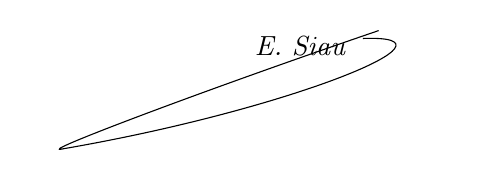
\begin{tikzpicture}[x=1cm,y=1cm]
\node[font=\itshape] at (3.1,.65) {\unsure{E. Siau}};
\draw (3.9,.75) .. controls (5.3,.8) and (3,-.15) .. (.1,-.65)
 .. controls (-.35,-.75) and (1.9,.1) .. (4.1,.85);
\end{tikzpicture}}
\uline{E. SIAU.}
% archive foliation: 42

\scanpage{44}
Genre de la courbe de Fermat $C_n$ (qui est une courbe
\inserted{plane} \deleted{\unsure{projective}} lisse de degré $n$)
\[
g_n=\frac{(n-1)(n-2)}2
\]
Le genre est 0 ssi $n=1,2$, il est 1 ssi $n=3$.
Pour $n=4$ il est 3, pour $n=6$ il est 10,
pour $n=12$ il est $55\ldots$

\rule{3cm}{0.4pt}

Considérons le cas $n=2$
\[
C_2:\quad x^2+y^2+z^2=0
\]
comme carte triangulée pondérée elle est formée de $4.2=8$ triangles,
chaque type de sommet intervient 2 fois, avec degré
$4$ \inserted{$(2.2)$} en chaque sommet.
Sauf erreur, c'est l'\uline{octaèdre} \inserted{sphérique}, dont le groupe des
automorphismes orientés est bien \inserted{$\simeq\unsure{\mathfrak S_4|\mathbb G_4}$}
d'ordre 24, et peut s'écrire comme produit $\frac12$ direct de
$\unsure{\mathfrak S_3|\mathbb G_3}$ par $(\mathbb Z_2)^2$ !
\figure{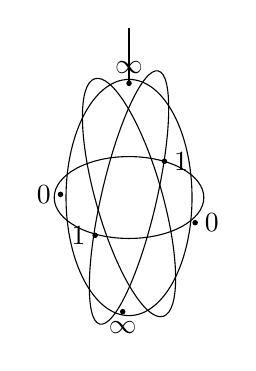
\begin{tikzpicture}[x=1cm,y=1cm]
\draw (0,0) ellipse (.8 and 1.5);
\draw (0,0) ellipse (.95 and .52);
\draw[rotate=-13] (0,0) ellipse (.35 and 1.65);
\draw[rotate=16] (0,0) ellipse (.42 and 1.57);
\draw (0,1.46)--(0,2.15);
\foreach \x/\y/\lab/\pos in {0/1.45/\infty/above,-.87/.04/0/left,.45/.46/1/right,.84/-.32/0/right,-.43/-.48/1/left,-.08/-1.45/\infty/below}{
\fill (\x,\y) circle (.035);\node[\pos] at (\x,\y) {$\lab$};}
\end{tikzpicture}}
% crop-candidate: scan 44
Divisant par les trois s-groupes $\mathbb F_2$ de
$\pi_2\simeq\mu_2^3/\mu_2$, on trouve les \inserted{3} revêtements
d'ordre 2 de $C_1:\simeq\mathbb P^1_{\mathbb Q}$ qui correspondent
au \deleted{dièdre} \inserted{monoèdre} \deleted{$\unsure{i=1}$}
(standard) et à ses transformés par $\unsure{\mathfrak S_3|\mathbb G_3}$.

\margin{\uline{NB} L'octaèdre est subdivision barycentrique du bi-èdre
(qui est autodual \unsure{\&|$*$} et a le type de ramification
\[
\begin{array}{ccc}2&2&2\\2&2&2\end{array}
\]
(cas particulier de celui du dièdre
\[
n\left\{\begin{matrix}2\\\vdots\\2\end{matrix}\right.\quad
\unsure{n}\left\{\begin{matrix}2\\\vdots\\2\end{matrix}\right.\quad
\begin{matrix}n\\n\end{matrix},\quad\text{pour }n=2),
\]
\unsure{ce qui} \uline{\unsure{entraîne|combinatoire}}, on le voit
de suite le rev. abélien universel
\inserted{\unsure{du monoèdre} \unsure{par} $\unsure{2}\unsure{\mathbin{-}}$}}
\figure{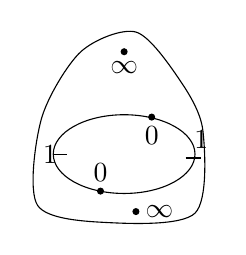
\begin{tikzpicture}[x=1cm,y=1cm]
\draw plot[smooth cycle] coordinates {(-1.1,-.65)(-1.05,.45)(-.55,1.3)(.15,1.55)(.7,.95)(1,.3)(.9,-.75)(-.2,-.87)};
\draw (0,0) ellipse (.9 and .5);
\fill (0,1.3) circle (.045) node[below] {$\infty$};
\fill (.15,-.73) circle (.045) node[right] {$\infty$};
\fill (.35,.47) circle (.045) node[below] {$0$};
\fill (-.3,-.47) circle (.045) node[above] {$0$};
\draw (-.9,0)--(-.73,0) node[left] {$1$};
\draw (.78,-.05)--(.98,-.05) node[above] {$1$};
\end{tikzpicture}}
% crop-candidate: scan 44
% The marginal note runs to and is physically clipped by the lower image edge.
% archive foliation: 43

\scanpage{45}
% Printed sheet upside down in the scan; transcribed after 180-degree rotation.
% One long diagonal cancellation stroke crosses the reused letter.
\deleted{
UNIVERSITE\\
DES SCIENCES ET TECHNIQUES\\
\uline{DU LANGUEDOC}\\
JFR/MD

Montpellier, le 22 Juin 1978

LE DIRECTEUR DE L'U. E. R. III

à

Mesdames et Messieurs les Membres\\
des Jurys des examens de l'U.E.R. III

Madame, Monsieur,

Le Conseil de l'U.E.R. III se permet de vous rappeler\\
qu'une réforme des maîtrises spécialisées est en cours, et que\\
tous les dossiers d'habilitation ou de reconduction devront parve-\\
nir au Ministère avant le 31 janvier 1979.

Pour faciliter sa tâche il vous serait reconnaissant de\\
bien vouloir lui indiquer si vous désirez que la maîtrise où vous\\
enseignez soit reconduite ou si vous souhaitez la modifier en tout\\
ou partie.

Il a pensé que les Jurys des différents certificats\\
étaient les plus propres à diffuser cette lettre auprès des ensei-\\
gnants qui s'estiment concernés. Il espère qu'ils voudront bien\\
examiner attentivement ce problème.

Il accueillera toute suggestion dont vous pourriez lui\\
faire part avant le 15 octobre 1978.

Il compte sur votre aide et vous prie de croire à tout\\
son dévouement.

Le Directeur de l'U.E.R. III,
\figure{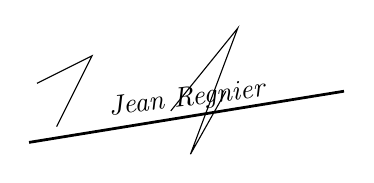
\begin{tikzpicture}[x=1cm,y=1cm]
\node[font=\itshape,rotate=7] at (2,.4) {\unsure{Jean Regnier}};
\draw[line width=1pt] (0,-.15)--(4,.5);
\draw (.1,.6)--(.8,.95)--(.35,.05);
\draw (1.8,.25)--(2.65,1.3)--(2.05,-.3)--(2.5,.5);
\end{tikzpicture}}
\uline{J.F. REGNIER}

\uline{N.B.} : Cette lettre a été transmise pour information aux Directeurs\\
d'U.E.R. et aux Membres du Conseil de l'U.E.R. III.
}
% archive foliation: 44
